\newcommand\pdeg{.\!\!\degree}
\newcommand\parcm{.\!\!'}

\section{Instrument}
\label{sec:instrument} %3

\begin{figure}
\begin{center}
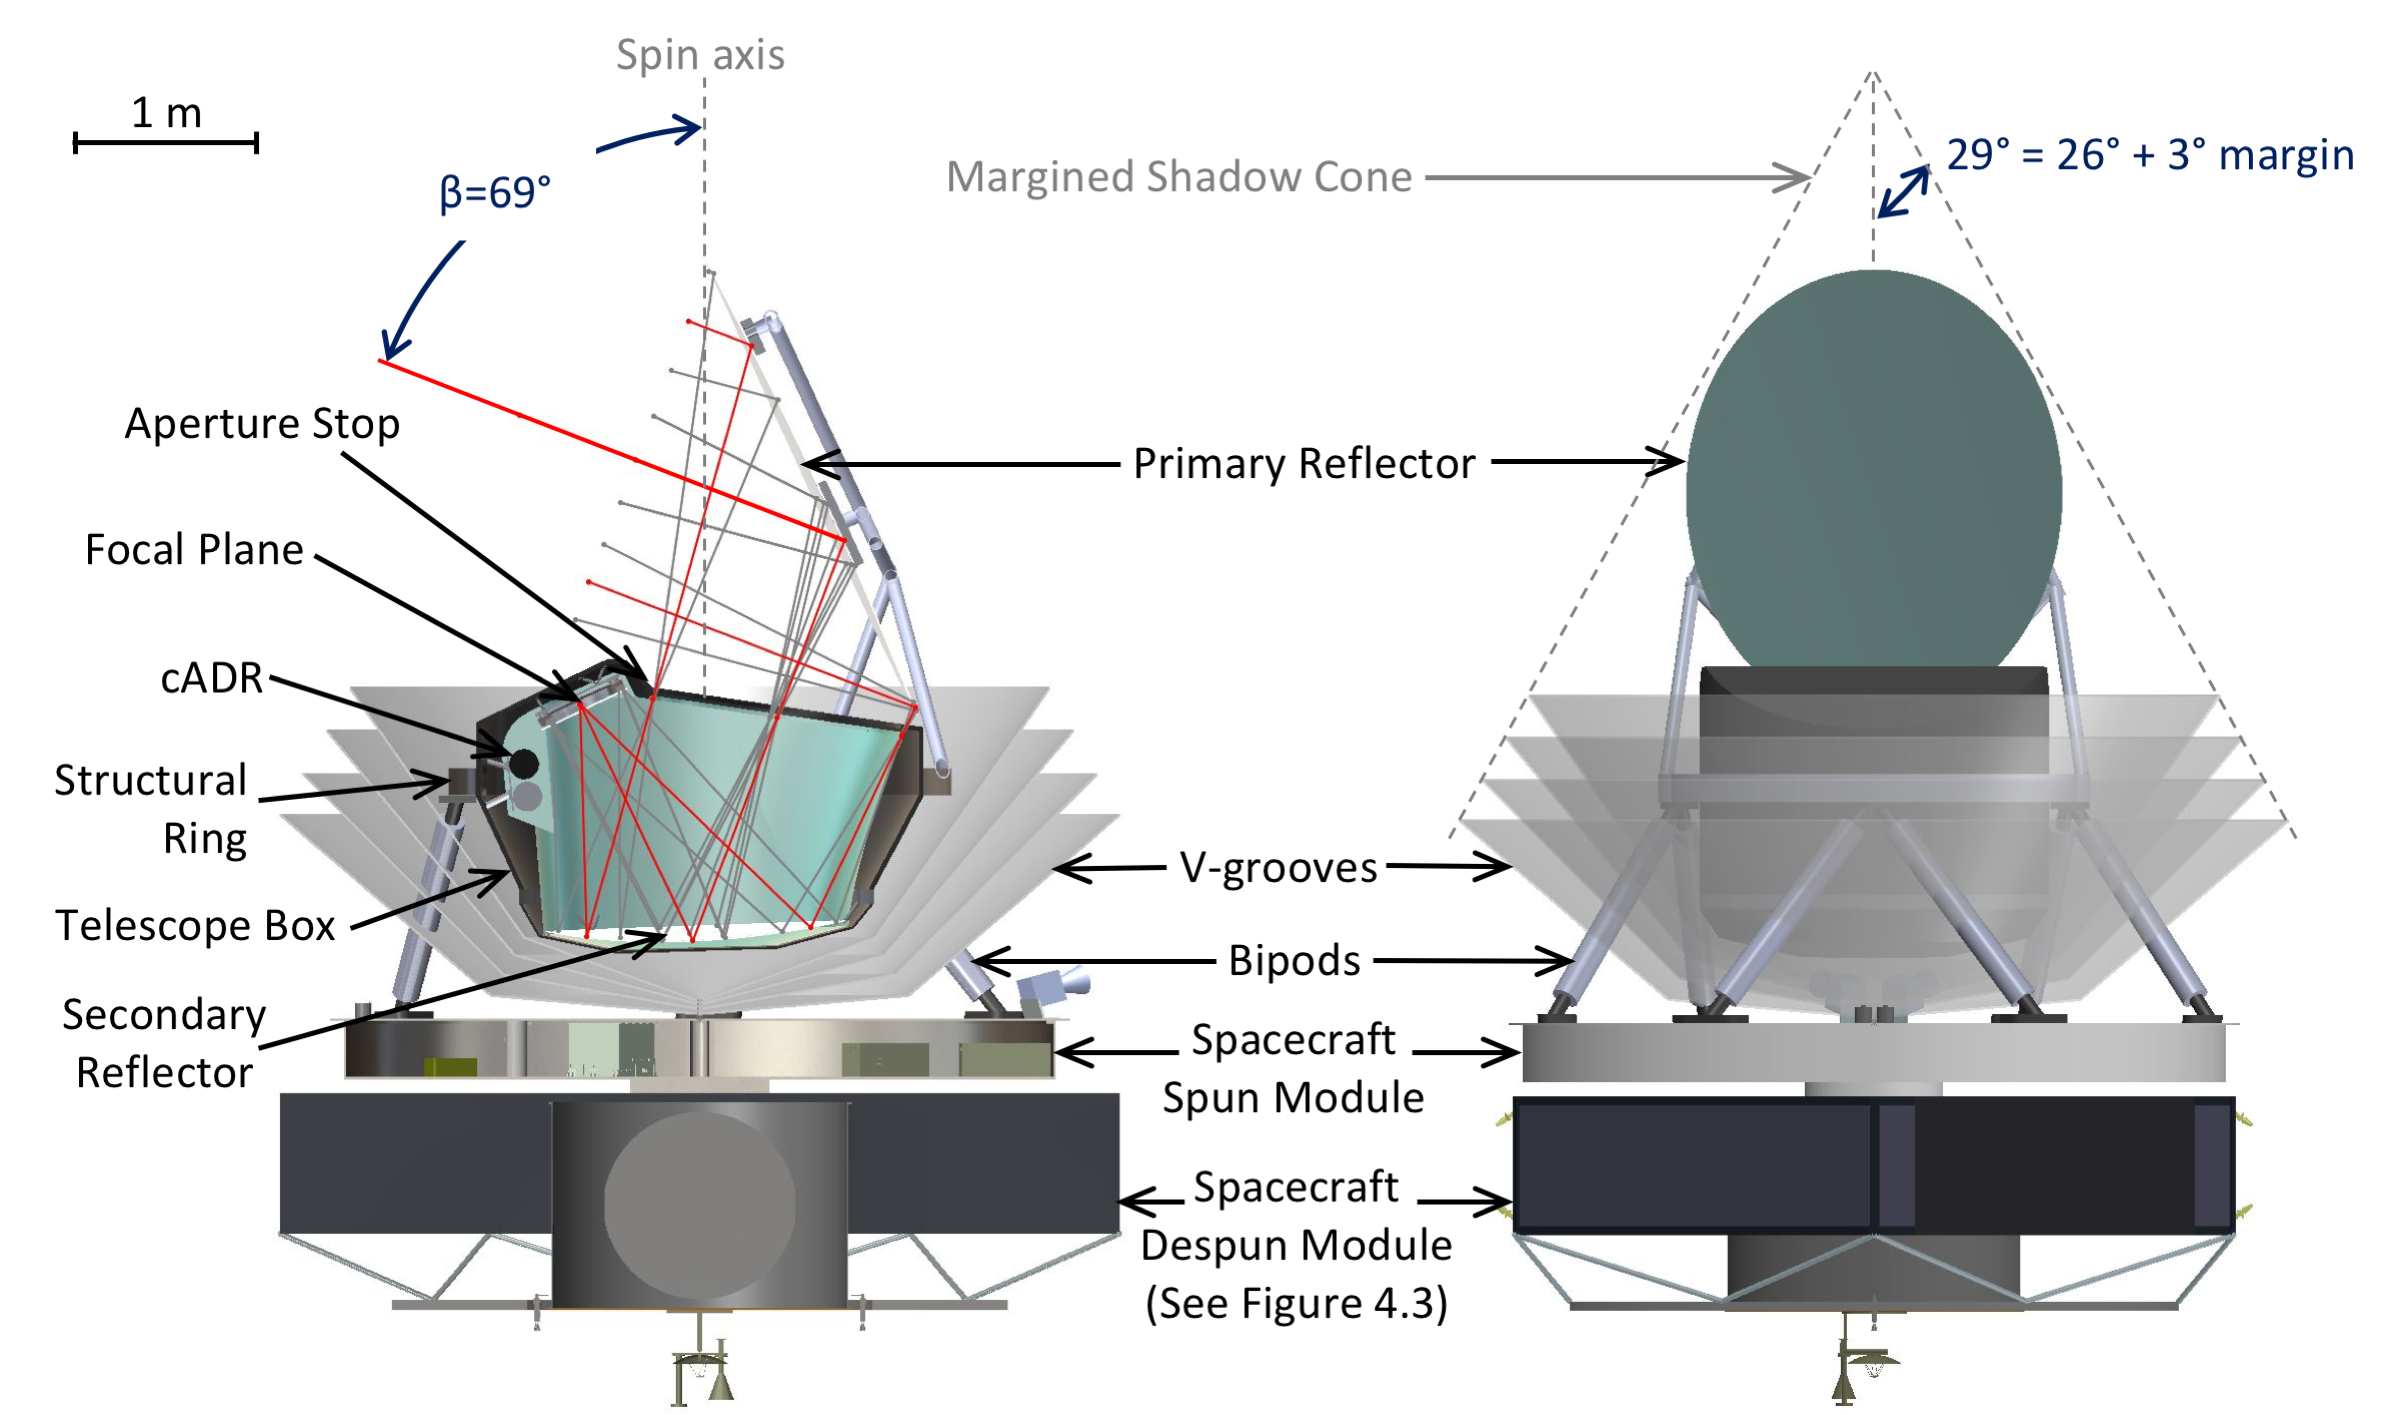
\includegraphics[width=6.25in]{figures/InstrumentCAD.png}
\vspace{-0.1in}
\caption{\captiontext
Detailed PICO instrument configuration. \textit{Left}: Side view in cross section. \textit{Right}: Front view with V-Groove assembly shown semi-transparent.  The spacecraft spun module accommodates warm instrument components: the 4\,K cooler compressor and drive electronics, the sub-K cooler drive electronics, and the detector warm readout electronics.
\label{fig:InstrumentCAD}}
\end{center}
\vspace{-0.15in}
\end{figure}

PICO meets all of its science-derived instrument requirements (Table~\ref{tab:STM}) with a single instrument: an imaging polarimeter with 21 logarithmically spaced frequency bands centered between 21 and 799\,GHz. The instrument is built around a two-reflector Dragone-style telescope (\S\,\ref{sec:telescope} and Fig.~\ref{fig:InstrumentCAD}) with an internal aperture stop between the primary and secondary. The focal plane is populated by 12,996 \ac{TES} bolometers (\S\,\ref{sec:focal_plane}) read out using a time-domain multiplexing scheme (\S\,\ref{sec:detector_readout}). The instrument employs a single science observing mode: fixed rate imaging while scanning the sky (\S~\ref{sec:survey_design}).

The instrument is configured inside the shadow of a V-groove assembly that thermally and optically shields it from the Sun (Fig.~\ref{fig:InstrumentCAD}). The V-groove assembly consists of 4 nested radiation shields that provide passive cooling (\S\,\ref{sec:radiative_cooling}). The sun shadow cone depicted in Fig.~\ref{fig:InstrumentCAD} is $29\degree$. The angle to the Sun during the survey, $\alpha = 26\degree$ (\S\,\ref{sec:survey_design} and Fig.~\ref{fig:MissionDesignFigure}), is supplemented with a margin of $3\degree$ to account for the radius of the sun ($0\pdeg25$), pointing control error, design margin, and alignment tolerances.

%A V-groove radiator assembly provides passive cooling (\S\,\ref{sec:radiative_cooling}). The instrument is configured inside the shadow of the V-grooves, thermally and optically shielded from the Sun. The sun shadow cone depicted in Fig.~\ref{fig:InstrumentCAD} is $29\degree$. The angle to the Sun during the survey, $\alpha = 26\degree$ (\S\,\ref{sec:survey_design} and Fig.~\ref{fig:MissionDesignFigure}), is supplemented with a margin of $3\degree$ to account for the radius of the sun ($0\pdeg25$), pointing control error, design margin, and alignment tolerances.

The V-groove assembly is attached to the bipod struts that support the instrument structural ring. The ring supports the primary reflector and telescope box. The telescope box contains the actively cooled components (\S\,\ref{sec:cadr}, \S\,\ref{sec:4kcooler}), including the secondary reflector, the focal plane and sub-kelvin adiabatic refrigerator structures. Just inside the box, a thermal liner serves as a cold optical baffle and aperture stop. Instrument integration and test (I\&T) are described in \S\,\ref{sec:iandt}.

During the survey, the instrument is spun at 1~rpm (\S\,\ref{sec:survey_design}). Spacecraft control is simplified by mounting the instrument on a spinning spacecraft module, while a larger non-spinning module houses most spacecraft subsystems (\S\,\ref{sec:spacecraft}). Instrument elements that act as heat sources are accommodated on the spinning module of the spacecraft.

\subsection{Telescope}
\label{sec:telescope} %3.1

The PICO telescope design is driven by a combination of science
requirements and physical volume limits. The science requirements are:
a large diffraction-limited field of view (DLFOV) sufficient to
support $\sim10^4$ detectors, arcminute resolution at 800\,GHz, low
spurious polarization, and low sidelobe response. All
requirements are met with PICO's 1.4\,m aperture modified open-Dragone
design. There are no moving parts in the PICO optical system.

\begin{figure}%[ht]
\parbox{4.0in}{
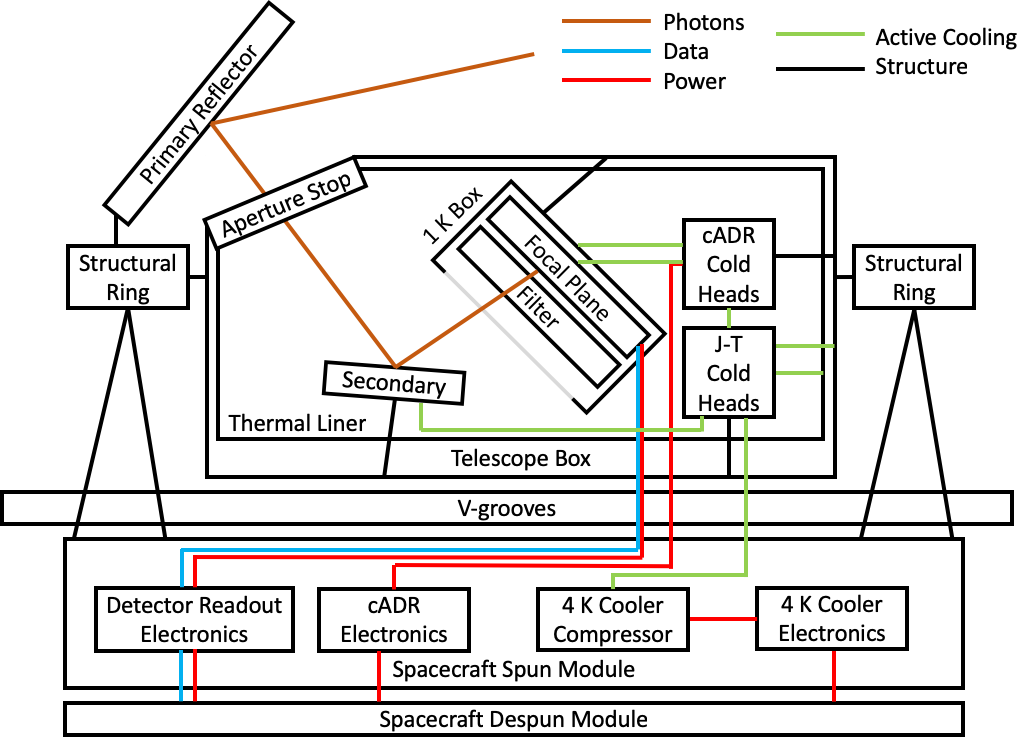
\includegraphics[width=4.0in]{images/ArchitectureBlockDiagram.png} }
\hspace{0.1in}
\parbox{2.3in}{
\caption{\captiontext
PICO instrument block diagram. Active coolers provide cooling to the 100\,mK focal plane, the surrounding 1\,K box, the 4.5\,K secondary reflector, and the 4.5\,K thermal liner that acts as a cold aperture stop. Data from the focal plane flows to (redundant, cross-strapped) warm readout electronics on the spun module of the spacecraft bus.
\label{fig:ArchitectureBlockDiagram} }  }
\end{figure}

The PICO optical design was selected following a trade study examining cross-Dragone, Gregorian Dragone, and open-Dragone designs~\citep{Young2018}.  The open-Dragone and crossed-Dragone offer more diffraction-limited focal plane area than the Gregorian Dragone~\citep{deBernardis2018}, and are able to support enough detectors to provide the required sensitivity. The open-Dragone does not require the massive and voluminous baffles that the cross-Dragone does, and hence can satisfy the aperture size requirement within the shadow cone.

PICO's initial open-Dragone design has been modified by adding an aperture stop and adding corrections to the primary and secondary reflectors to enlarge the DLFOV. The detailed geometric parameterization of the PICO optical design is described in~\citep{Young2018}. The primary reflector (270\,cm $\times$ 205\,cm) is passively cooled and the secondary reflector (160\,cm $\times$ 158\,cm) is actively cooled. The highest frequency (900\,GHz) sets the surface accuracy requirement of the reflectors at $\sim \lambda/14 =24\,\mu{\rm m}$. The focal ratio is 1.42. The slightly concave focal surface, which has a radius of curvature of 4.55~m, is telecentric to within $0\pdeg12$ across the entire FOV.

%\comblue{what about the reflector material?}
An actively cooled circular aperture stop between the primary and secondary reflectors reduces detector noise and shields the focal plane from stray radiation. Stray-light analysis of the PICO open-Dragone design using GRASP confirms that the focal plane is protected from direct view of the sky, and that spillover past the primary is suppressed by 80~dB relative to the main lobe for both co-pol and cross-pol beams. Detailed baffle design will be performed during mission formulation.


% \begin{figure}
% \begin{center}
% 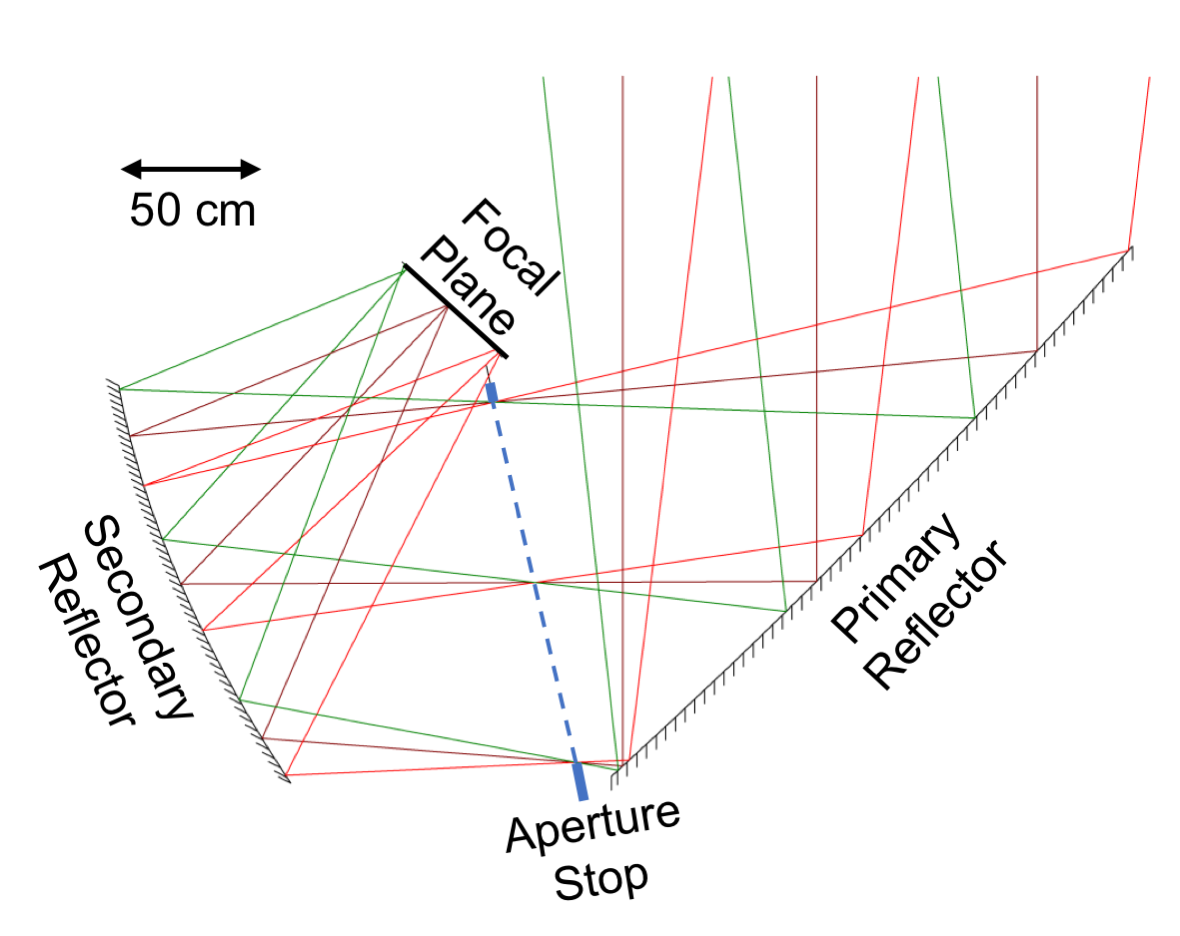
\includegraphics[width=3in]{figures/OpticsDiagram.png}
% \caption{The optical system is compact.\label{fig:OpticsDiagram}}
% \end{center}
% \end{figure}

\subsection{Focal plane}
\label{sec:focal_plane} %3.2
%
% wrap version of figure 3.3.  Unwrapped version is below.
\begin{wrapfigure}{r}{0.45\textwidth}
\vskip -8pt
\hfill
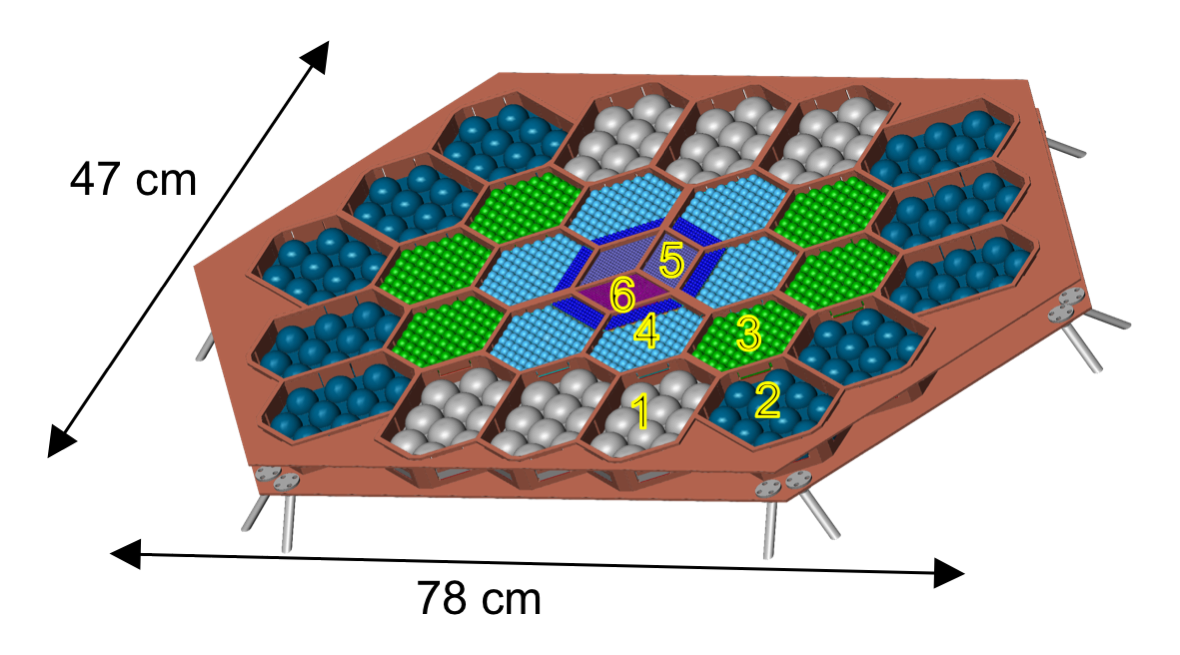
\includegraphics[width=0.45\textwidth]{figures/FocalPlaneMechanical.png}
\vskip -2pt
\caption{\captiontext PICO focal plane. Detectors are fabricated on six types of tiles (shown numbered and colored as in Table~\ref{tab:focal_plane}). The wafers are located on the focal plane such that higher frequency bands, which require better optical performance, are placed nearer to the center.\label{fig:FocalPlaneMechanical}}
\end{wrapfigure}


PICO's focal plane is populated by an %imaging
array of \ac{TES} bolometers operating in 21 %overlapping
frequency bands, each with 25\% fractional bandwidth, and band centers ranging from 21 to 799~GHz.
Polarimetry is achieved by differencing the signals from pairs of two co-pointed bolometers that are sensitive to two orthogonal polarization states. %\comblue{polarimetry is incomplete; need to elaborate more}
A conceptual layout of the PICO focal plane is shown in Fig.~\ref{fig:FocalPlaneMechanical} and detailed in Table~\ref{tab:focal_plane}.

% \begin{figure}
% \centering
% \begin{minipage}{0.49\textwidth}
% \centering
% 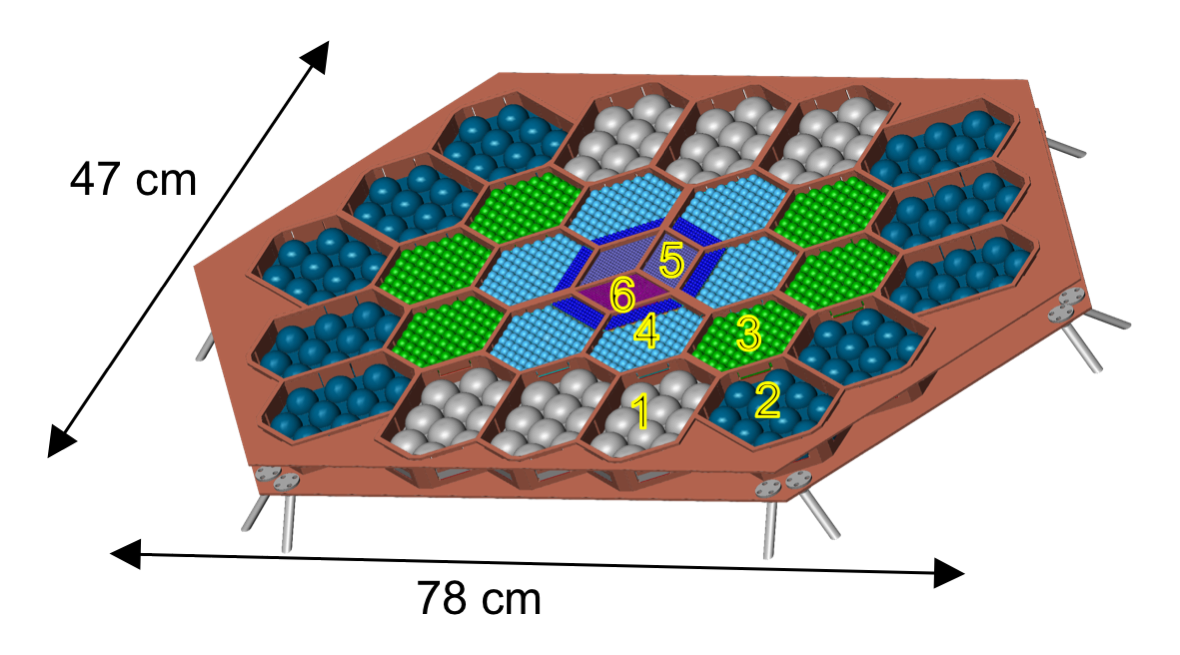
\includegraphics[width=\textwidth]{figures/FocalPlaneMechanical.png}
% \caption{\captiontext PICO focal plane. Detectors are fabricated on six types of tiles (shown numbered and colored as in Table~\ref{tab:focal_plane}). The wafers are located on the focal plane such that higher frequency bands, which require better optical performance, are placed nearer to the center.\label{fig:FocalPlaneMechanical}}
% \end{minipage}
% \hfill
% \begin{minipage}{0.49\textwidth}
% \centering
% \captionsetup{type=table}
% \caption{\captiontext PICO makes efficient use of the focal area with multichroic pixels (three bands per pixel, \S\,\ref{sec:low_freq_det}). The sampling rate is based on the smallest beam (Table~\ref{tab:bands}), with 3 samples per FWHM at a scan speed $(360\degree/{\rm min})\sin(\beta=69\degree) = 336\degree/{\rm min}$. Scaling from suborbital experience, we anticipate that TES bolometers can support these sampling rates with a factor of $\sim4\times$ margin.\label{tab:focal_plane}}{%
% \begingroup
% \definecolor{A}{RGB}{209, 209, 209}
% \definecolor{B}{RGB}{64, 128, 159}
% \definecolor{C}{RGB}{112, 208, 85}
% \definecolor{D}{RGB}{109, 196, 232}
% \definecolor{E}{RGB}{32, 49, 184}
% \definecolor{F}{RGB}{119, 120, 199}
% \definecolor{G}{RGB}{235, 92, 243}
% %\openup 5pt
% \newdimen\tblskip \tblskip=5pt
% \nointerlineskip
% \vskip -6mm
% \footnotesize %\footnotesize
% \setbox\tablebox=\vbox{
%     \newdimen\digitwidth
%     \setbox0=\hbox{\rm 0}
%     \digitwidth=\wd0
%     \catcode`*=\active
%     \def*{\kern\digitwidth}
% %
%     \newdimen\signwidth
%     \setbox0=\hbox{+}
%     \signwidth=\wd0
%     \catcode`!=\active
%     \def!{\kern\signwidth}
% %
% \halign to \textwidth{
% \hfil#\hfil\tabskip=0.6em plus 0.6em&
% \hfil#\hfil&
% \hfil#\hfil&
% \hfil#\hfil&
% \hfil#\hfil&
% \hfil#\hfil\tabskip=0pt\cr
% \noalign{\doubleline}
% \omit \hfil Tile\hfil&&Pixels/&Pixel&Bandcenters&Sampling\cr
% \omit \hfil type\hfil&$N_{\rm tile}$&tile&type&[GHz]&rate [Hz]\cr
% \noalign{\vskip 3pt\hrule\vskip 5pt}
% 1&6&10&\colorbox{A}{A}&21, 30, 43&45\cr
% \noalign{\vskip 5pt\hrule height 0.2pt\vskip 3pt}
% 2&10&10&\colorbox{B}{\textcolor{White}B}&25, 36, 52&55\cr
% \noalign{\vskip 5pt\hrule height 0.2pt\vskip 3pt}
% 3&6&61&\colorbox{C}{C}&62, 90, 129&136\cr
% \noalign{\vskip 5pt\hrule height 0.2pt\vskip 3pt}
% 4&6&85&\colorbox{D}{D}&75, 108, 155&163\cr
% \omit&\omit&80&\colorbox{E}{\textcolor{White}E}&186, 268, 385&403\cr
% \noalign{\vskip 5pt\hrule height 0.2pt\vskip 3pt}
% 5&2&450&\colorbox{F}{\textcolor{White}F}&223, 321, 462&480\cr
% \noalign{\vskip 5pt\hrule height 0.2pt\vskip 3pt}
% 6&1&220&\colorbox{G}{G}&555&917\cr
% \omit&\omit&200&\colorbox{G}{H}&666\cr
% \omit&\omit&180&\colorbox{G}{I}&799\cr
% \noalign{\vskip 5pt\hrule\vskip 3pt}
% } % close halign
% } % close vbox
% \endPlancktable
% \endgroup
% }
% \end{minipage}
% \end{figure}

% version of 3.3 with text beside image.
% \begin{figure}
% \parbox{3in}{\centering
% 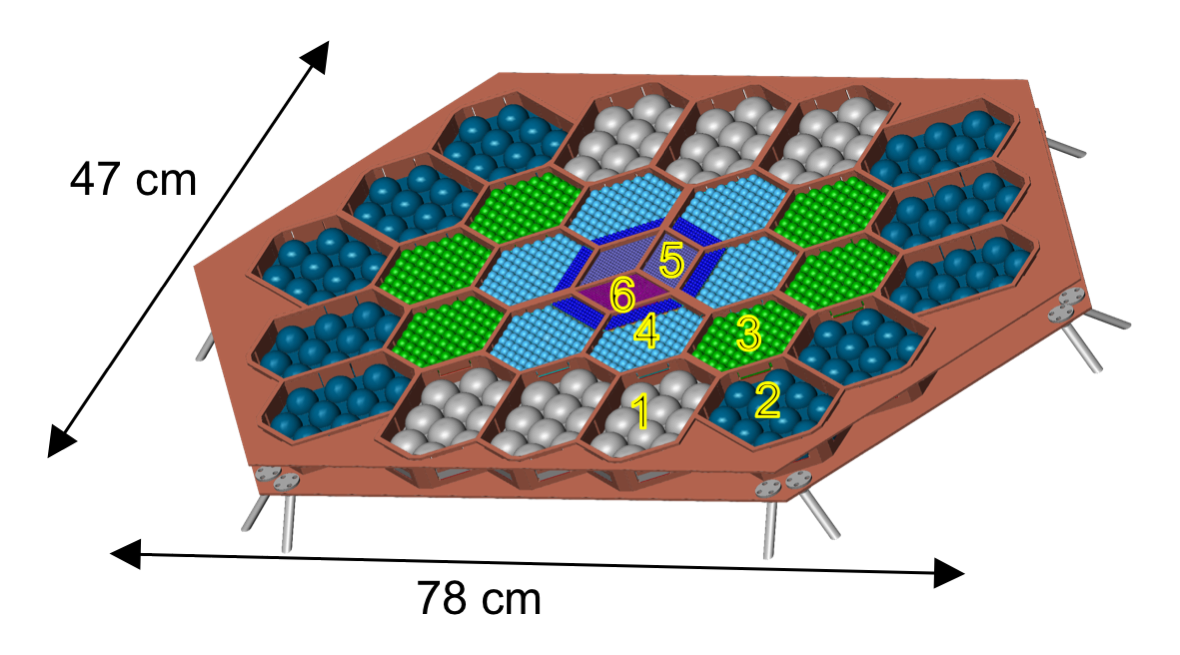
\includegraphics[width=3in]{figures/FocalPlaneMechanical.png}
% }
% \parbox{3.5in}{\centering
% \caption{\captiontext
% PICO focal plane. Detectors are fabricated on six types of tiles (shown numbered and colored as in Table~\ref{tab:focal_plane}). The wafers are located on the focal plane such that higher frequency bands, which require better optical performance, are placed nearer to the center.\label{fig:FocalPlaneMechanical}}
% }
% \end{figure}

Bolometers operating in the mm/sub-mm wave band are photon-noise limited. Therefore, increase in sensitivity is achieved through an increase in detector count. The PICO focal plane has 12,996 detectors, 175 times the number flown aboard \planck\ thereby providing a breakthrough increase in sensitivity with a comparably sized telescope. This breakthrough is enabled by development and demonstration in suborbital projects, which now commonly operate arrays of $10^3$--$10^4$ detectors (\S\,\ref{sec:technology_maturation}).

\subsubsection{21--462\,GHz Bands}
\label{sec:low_freq_det} % 3.2.1
%
%\input tables/table3.1_wrap.tex

Several optical coupling technologies have matured over the past ten
years to efficiently use focal plane area: horns with ortho-mode
transducers (OMTs) \citep{Duff2016}, lithographed antenna arrays
\citep{BICEP2015}, and sinuous antennas under lenslets
\citep{Edwards2012}. Horn-coupling and sinuous
antenna/lenslet-coupling deliver quantum efficiency $>70\,\%$ over
more than an octave of bandwidth, which can be partitioned into two
or three colors per pixel.  Alternatively, antenna-array coupling has
only demonstrated single-color pixels to date, but uniformly
illuminated feeds enable much smaller pixels and therefore more
densely packed focal planes.
% Amy:I'd very much like to be able to add this sentence if its true,
% but I haven't seen the antenna-array analysis, and it isn’t yet
% included in 5.5: “Any of these technologies could be used to deliver
% dramatic increases in instrument sensitivity relative to the Planck
% mission (§5.5).”


The PICO baseline focal-plane design
employs three-color sinuous antenna/lenslet-coupling \citep{Suzuki2014}
for the 21--462\,GHz bands. Niobium microstrips mediate the signals
between the antenna and detectors, and partition the feed's wide
continuous bandwidth into three narrow channels using integrated
micro-machined filter circuits \citep{OBrient2013}. The technology
maturation required for PICO is described in \$\,\ref{sec:bolometers}.

% The majority of the PICO FOV is populated with multichroic pixels (MCPs)
% \citep{Suzuki2014,Datta2014}, which make optimal use of the focal
% plane area by feeding three photometric bands from a common broad-band
% antenna, with two single-polarization bolometers per band and
% therefore six bolometers per pixel.

% Several competing optical coupling technologies have matured over the
% past ten years using horn-coupling \citep{Duff2016}, antenna-array
% coupling \citep{BICEP2015}, and sinuous antenna/lenslet-coupling
% \citep{Edwards2012}, delivering quantum efficiency $> 70\,\%$ over more than
% an octave of bandwidth. Pixel size, number, and spacing are relatively
% agnostic to the coupling scheme, so multiple options are open to PICO
% (technology maturation plan described in
% \S\,\ref{sec:bolometers}). For all of these schemes, niobium
% microstrips mediate the signals between the antenna and detectors, and
% partition the feed's wide continuous bandwidth into narrow channels
% using integrated micro-machined filter circuits \citep{OBrient2013}.

\subsubsection{555--799\,GHz Bands}
\label{sec:high_freq_det} % 3.2.2
%
\input tables/table3.1_wrap.tex

PICO's highest three frequency channels are beyond the niobium superconducting band-gap, rendering microstrip filters a poor solution for defining the optical passband. In this regime, PICO instead measures a single band with each pixel using feedhorn-coupled polarization-sensitive bolometers. Radiation is coupled through horns directly to an absorber in the throat of a waveguide. TES bolometers detect the incident power.  The waveguide cut-off defines the lower edge of the band, and quasi-optical metal-mesh filters define the upper edge. Numerous experiments have successfully used similar approaches~\citep{Shirokoff2011,Bleem2012,Turner2001}. The technology maturation required for PICO is described in \S\,\ref{sec:dev_arrays}.

\input tables/table3.2.tex

\subsubsection{Sensitivity}
\label{sec:sensitivity} %3.2.3

PICO's Current Best Estimate (CBE) sensitivity meets the requirements of the baseline mission with \hbox{$>40\,\%$} margin (Table~\ref{tab:bands}).
%\comblue{this is an odd statement. need to rework}

We developed an end-to-end noise model of the PICO instrument to predict mission sensitivity and provide a metric by which to evaluate mission design trades. The model includes four noise sources per bolometer: photon, phonon, Johnson, and readout (from both cold and warm readout electronics). To validate our calculations, we compared two independent software packages that have been validated with several operating CMB instruments. The calculations agreed within 1\% both for individual noise terms and for overall mission noise. A detailed description of the PICO noise model and its inputs is available in~\citet{Young2018}; small differences between that publication and Table~\ref{tab:bands} are due to refinements of the primary mirror and stop temperatures.
%\comblue{need to explain better}

% removed TES Johnson

Laboratory experiments have demonstrated that TES bolometers can be made background-limited in the low loading environment they would experience at L2~\citep{Beyer2012}. For PICO, the primary contributor to noise is the optical load. The sources of optical load are the CMB, reflectors, aperture stop, and low-pass filters. The CMB and stop account for at least 50\% of the optical load at all frequencies up to and including 555~GHz. At higher bands emission from the primary mirror dominates.
%The CMB gives more than half the load in the middle and upper bands of the multichroic pixels, but the stop dominates the load in the lowest band of each pixel.

The sensitivity model assumes white noise at all frequencies. Sub-orbital submillimeter experiments have demonstrated TES detectors that are stable to at least as low as 20\,mHz \citep{Rahlin2014}, meeting the requirements for PICO's scan strategy (\S\,\ref{sec:survey_design}). %\comblue{are we saying anything about 1/f? are we saying anything about yield? Is the observing time consistent with Young et al?}

\subsection{Detector Readout}
\label{sec:detector_readout} %3.3

Suborbital experiment teams over the past ten years have chosen to use voltage-biased TESs because their current readout scheme lends itself to Superconducting Quantum Interface Device (SQUID) based multiplexing. Multiplexing reduces the number of wires to the cryogenic stages and thus the total thermal load that the cryocoolers must dissipate. This approach also simplifies the instrument design.

In the multiplexing circuitry, SQUIDs function as low-noise amplifiers and cryogenic switches. The current baseline for PICO is to use a time-domain multiplexer (TDM), which assigns each detector's address in a square matrix of simultaneously read columns, and sequentially cycles through each row of the array \citep{Henderson2016}. The PICO baseline architecture uses a matrix of 128 rows and 102 columns.
%, requiring some technology maturation (\S\,\ref{sec:multiplexing}).
The thermal loading on the cold stages from the wire harnesses is subdominant to conductive loading through the mechanical support structures.

Because SQUIDs are sensitive magnetometers, suborbital experiments
have developed techniques to shield them from Earth's magnetic field
using highly permeable materials and superconducting materials
\citep{Hui2018}.  Total suppression factors better than $10^7$ have
been demonstrated for dynamic magnetic fields \citep{Runyan2010}. PICO
will use these demonstrated techniques to shield SQUID readout chips
from the ambient magnetic environment, which is 20,000 times smaller
than near Earth, as well as from fields generated by on-board
components including the cADR (\S\,\ref{sec:cadr}). The cADR is
delivered with its own magnetic shielding which reduces the field to
less than 0.1\,G (less than that experienced by suborbital
experiments).

SQUIDS are also sensitive to radio-frequency interference
(RFI). Several suborbital experiments have demonstrated RFI shielding
using aluminized mylar wrapped at cryogenic stages to form a Faraday
cage around the SQUIDs \citep{Kermish2012,EBEX2018,BICEP2014}.
 Cable shielding extends the Faraday cage to
the detector warm readout electronics.

Redundant warm electronics boxes perform detector readout and
instrument housekeeping using commercially available radiation
hardened analog-to-digital converters (ADCs), requiring 75\,W total.
The readout electronics compress the data before delivering them to
the spacecraft, requiring an additional 15\,W. PICO detectors produce
a total of 6.1\,Tbits/day assuming 16\,bits/sample, sampling rates
from Table~\ref{tab:focal_plane}, and bolometer counts from
Table~\ref{tab:bands}. \textit{Planck} HFI typically achieved
4.7$\times$ compression in flight with information loss increasing
noise by $\sim10\,\%$ \citep{Pajot2018,PlanckHFI2011}. Suborbital work
has demonstrated 6.2$\times$ lossless compression
\citep{EBEX2017}. PICO assumes 4$\times$ lossless compression.

\subsection{Thermal}
\label{sec:thermal} %3.4

Like the \planck -HFI instrument, PICO's focal plane is maintained at 0.1~K to ensure low detector noise while implementing a readily available technology~(\S\,\ref{sec:cadr}). To minimize detector noise due to instrument thermal radiation, the aperture stop and reflectors are cooled using both active and radiative cooling (\S\,\ref{sec:4kcooler}, \S\,\ref{sec:radiative_cooling}, Fig.~\ref{fig:ArchitectureBlockDiagram}).  All thermal requirements are met with robust margins (Table~\ref{tab:cooler}).

\input tables/table3.3.tex

\subsubsection{cADR Sub-Kelvin Cooling}
\label{sec:cadr} %3.4.1

A multi-stage continuous adiabatic demagnetization refrigerator (cADR) maintains the PICO focal plane at 0.1~K and the surrounding enclosure, filter, and readout components at 1~K. The cADR employs three refrigerant assemblies operating sequentially to absorb heat from the focal plane at 0.1~K and reject it to~1~K. Two additional assemblies, also operating sequentially, absorb this rejected heat at~1~K, cool other components to 1~K, and reject heat at~4.5~K. This configuration provides continuous cooling with small temperature variations at both the 0.1~K and 1~K. Heat straps connect the two cADR cold sinks to multiple points on the focal plane assembly,
%\comor{was 'focal plane assembly' defined? isn't it at 0.1K?}
which has high thermal conductance paths built in, to provide spatial temperature uniformity and stability during operation. The detector arrays are thermally sunk to the mounting frame.  Heat loads in the range of 30~$\mu$W at 0.1~K and 1~mW at 1~K (time-average) are within the capabilities of current cADRs developed by GSFC (\S~\ref{sec:heritage})~\citep{Shirron2012,Shirron2016}. The PICO sub-kelvin heat loads are estimated at less than half of this capability (Table~\ref{tab:cooler}).
%\comblue{this paragraph doesn't say anything about the maturity of the multiple stage cADR, and about flight heritage. It should, even if to point to later paragraphs.}

\subsubsection{4.5~K Cooler}
\label{sec:4kcooler} %3.4.2

A cryocooler system similar to that used on JWST to cool the MIRI detectors~\citep{Durand2008,Rabb2013} removes the heat rejected from the cADR and cools the aperture stop and secondary reflector to 4.5~K. Both NGAS (which provided the MIRI coolers) and Ball Aerospace have developed such coolers under the NASA-sponsored Advanced Cryocooler Technology Development Program~\citep{Glaister2006}. NGAS and Ball use slightly different but functionally-equivalent hardware approaches. A 3-stage precooler provides $\sim16$~K precooling to a separate circulated-gas loop.
%driven by a similar compressor but modified for DC flow \comblue{very technical; is the reader supposed to follow this? is the difference between the ngas and ball relevant?}.
The circulated-gas loop utilizes Joule--Thomson (J-T) expansion, further cooling the gas to 4.5~K.
The J-T expansion point is located close to the cADR heat rejection point and provides it the lowest temperature. Subsequently, the gas flow intercepts heat conducted to the focal plane enclosure, then cools the aperture stop and the secondary reflector before returning to the circulation compressor.  %Model-based projections indicate that the coolers delivered for MIRI could meet the PICO 4.5~K heat lift requirement with more than $100\,\%$ margin with these straightforward modifications: replacement of the $^4$He gas used for MIRI's J-T  with $^3$He; and resizing the $^3$He heat exchangers to take advantage of the different gas properties.

NGAS and Ball are actively working on increasing the flow rate and compression ratio of the J-T compressor,  which should result in higher system efficiency and greater heat-lift relative to the current MIRI cooler. 
%, giving an additional path for obtaining margin above the PICO requirement. 
NGAS uses $^4$He as the circulating gas, as was used for MIRI. Ball uses a somewhat larger compressor and $^3$He as the circulating gas. Both employ re-optimized heat exchangers. The NGAS project has completed PDR-level development, and is expected to reach CDR well before PICO begins Phase-A. The projected performance of this cooler is shown in Fig.~\ref{fig:CoolerFigure}; it gives 100~mW at 250~W input power, which is more than 100\,\% heat lift margin relative to PICO's requirements (Table~\ref{tab:cooler}). For PICO we assumed an input power of 350~W.

The entire precooler assembly and the J-T circulator compressor are located on the warm spacecraft spun module (Fig.~\ref{fig:ArchitectureBlockDiagram}).
%, with relatively short tubing lengths conducting the gas flow from the precooling point to the J-T expansion point.
All waste heat rejected by the cooler compressors and drive electronics is transferred to the spacecraft heat rejection system. Unlike JWST, the PICO cooler does not require deployment of the remote cold head.

%A 3-stage precooler (acoustic Stirling by NGAS or mechanical Stirling by Ball) provides $\sim16$~K precooling to a separate circulated-gas loop driven by a similar compressor modified for DC flow \comblue{very technical; is the reader supposed to follow this? is the difference between the ngas and ball relevant?}. The circulated-gas loop utilizes Joule--Thomson (J-T) expansion, further cooling the gas to 4.5~K. The entire precooler assembly and the J-T circulator compressor are located on the warm spacecraft spun module (Fig.~\ref{fig:ArchitectureBlockDiagram}), with relatively short tubing lengths conducting the gas flow from the precooling point to the J-T expansion point. All waste heat rejected by the cooler compressors and drive electronics is transferred to the spacecraft heat rejection system. Unlike JWST, the PICO cooler does not require deployment of the remote cold head.

%The J-T expansion point is located close to the cADR heat rejection point, thereby providing the lowest temperature to the cADR. Subsequent to cooling the cADR, the gas flow intercepts conducted heat to the focal plane enclosure, then cools the aperture stop and the secondary reflector before returning in counterflow to the circulation compressor.  Model-based projections indicate that the coolers delivered for MIRI could meet the PICO 4.5~K heat lift requirement with more than $100\,\%$ margin with minimal changes: the replacement of the $^4$He gas used for MIRI with $^3$He, plus resizing of the gas counterflow heat exchangers to take advantage of the $^3$He properties. \comblue{have we thought through about the change in gas? is it obvious that no other changes will be required as a consequence of the change in gas type?}

\begin{figure}
\parbox{3.5in}{\centering
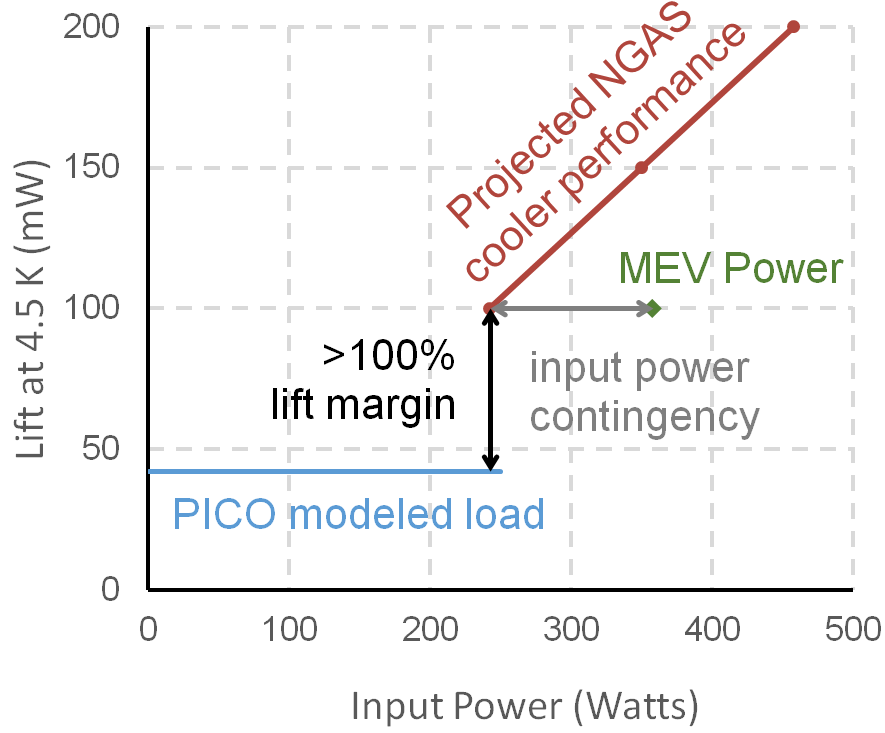
\includegraphics[width=2.6in]{figures/CoolerFigure.png} }
\parbox{3.0in}{
\caption{\captiontext
Projected performance of the NGAS cooler using a multi-stage
compressor and $^4$He circulating gas~\citep{Rabb2013} meets PICO's requirements
with $>100\,\%$ margin. PICO requires heat lift of 42 mW at 4.5~K (Table~\ref{tab:cooler}). With 250~W of input power the NGAS cooler is projected to provide 100~mW of heat lift. We conservatively specify a maximum expected value (MEV) of 350~W as the compressor's input power, giving 100~W of additional input power contingency.
  \label{fig:CoolerFigure}} }
\vspace{-0.15in}
\end{figure}

%There is a second approach that will meet the PICO requirements without assuming modifications of the MIRI cooler.

%which requires less modification to achieve comparable performance,
%These improvements entail the implementation of well-known techniques (standard thermal engineering) \comblue{what does this sentence mean?}.
%The NGAS project has completed PDR-level development, and is expected to reach CDR level well before PICO begins PhaseA. The projected performance of this cooler is shown in Fig.~\ref{fig:CoolerFigure}; it gives more than 100\% heat lift at 250~W input power. For PICO we assumed a maximum expected input power of 350~W. The Ball approach started with a larger compressor, required less modification to achieve comparable performance, and eliminated the cold bypass-precooling valve that was problematic for MIRI. \comblue{must we mention problematic valves?} The Ball approach uses $^3$He, while the NGAS approach uses $^4$He. Both employ re-optimized gas heat exchangers (trivial engineering changes). \comblue{what does this mean?}

%It is highly likely that a better solution will be available before Phase~A. \comblue{why do we need a better solution? do you mean a cooler with even larger margin?} NGAS and Ball are actively working on increasing the flow rate and compression ratio of the J-T compressor, which should result in significantly higher system efficiency, and in greater heat-lift margin above the PICO requirement. These improvements entail the implementation of well-known techniques (standard thermal engineering) \comblue{what does this sentence mean?}. The NGAS multi-stage J-T compressor has completed PDR-level development, and is expected to reach CDR level well before needed for PICO. Projected performance is shown in Fig.~\ref{fig:CoolerFigure}. The Ball approach started with a larger compressor, required less modification to achieve comparable performance, and eliminated the cold bypass-precooling valve that was problematic for MIRI. \comblue{must we mention problematic valves?} The Ball approach uses $^3$He, while the NGAS approach uses $^4$He. Both employ re-optimized gas heat exchangers (trivial engineering changes). \comblue{what does this mean?}


\subsubsection{Radiative Cooling}
\label{sec:radiative_cooling} %3.4.3

A set of four V-groove radiators provides passive cooling. This is standard technology, with origins dating to more than 30 years ago~(\S~\ref{sec:heritage}). The outermost of the four V-groove shields shadows the interior shields from the Sun. The V-grooves radiate to space, each reaching successively cooler temperatures.
%\comblue{can we be quantitative?}
The V-groove assembly provides a cold radiative environment to the primary reflector, structural ring, and telescope box, so radiative loads on those elements are smaller than the conductive loads through the mechanical support structures.
%\comblue{shouldn't we show evidence that say radiative cooling has been worked out successfully before.? }


\subsection{Instrument Integration and Test}
\label{sec:iandt} % 3.5

PICO instrument I\&T planning benefits greatly from heritage
experience with the \textit{Planck} HFI instrument \citep{ Pajot2010}.

PICO screens detector wafer performance prior to selection of
flight wafers and focal plane integration. The cADR and 4\,K
cryocooler are qualified prior to delivery. The relative alignment
of the two reflectors under thermal contraction is
photogrammetrically verified in a thermal vacuum (TVAC) chamber.

PICO integrates the flight focal plane assembly and flight cADR in
a dedicated sub-kelvin cryogenic testbed. Noise, responsivity, and focal-plane
temperature stability are characterized using a representative
optical load for each frequency band (temperature-controlled
blackbody). Polarimetric and spectroscopic calibration are
performed.

The focal plane is integrated with the reflectors and structures, and
alignment verified photogrammetrically at cold temperatures in a TVAC
chamber.  The completely integrated observatory (instrument and
spacecraft bus) is tested in TVAC to measure parasitic optical loading
from the instrument, noise, microphonics, and radio-frequency
interference (RFI). The observatory is 4.5\,m in diameter and 6.1\,m
tall, with no deployables.

%\newpage
\section{Design Reference Mission}
\label{sec:design_reference} %4
The PICO design reference mission is summarized in Table~\ref{tab:mission_parameters}.

\subsection{Concept of Operations}
\label{sec:operations} %4.1
%
\input tables/table4.1_wrap.tex
%
The PICO concept of operations is similar to that of the successful
\textit{WMAP} \citep{Bennett2003} and \textit{Planck} \citep{Tauber2010} missions. After launch,
PICO cruises to a quasi-halo orbit around the Earth--Sun L2 Lagrange point
(\S\,\ref{sec:mission_design}). A two-week decontamination period is followed by
instrument cooldown, lasting about two months. After in-orbit checkout is complete, PICO begins
the science survey.

PICO has a single science observing mode, surveying the sky
continuously for 5 years using a pre-planned repetitive survey pattern
(\S\,\ref{sec:survey_design}). Instrument data are compressed and stored on-board, then
returned to Earth in daily 4-hr Ka-band science downlink passes
(concurrent with science observations). Because PICO is observing
relatively static Galactic, extragalactic, and cosmological targets,
there are no requirements for time-critical observations or data
latency. Presently, there are no plans for targets of opportunity or
guest observer programs during the prime mission. The PICO instrument
does not require cryogenic consumables (as the \textit{Planck} mission did),
permitting consideration of significant mission extension beyond the prime
mission.


\begin{figure}[!b]
  \begin{minipage}[b]{0.29\textwidth}
    \begin{center}
    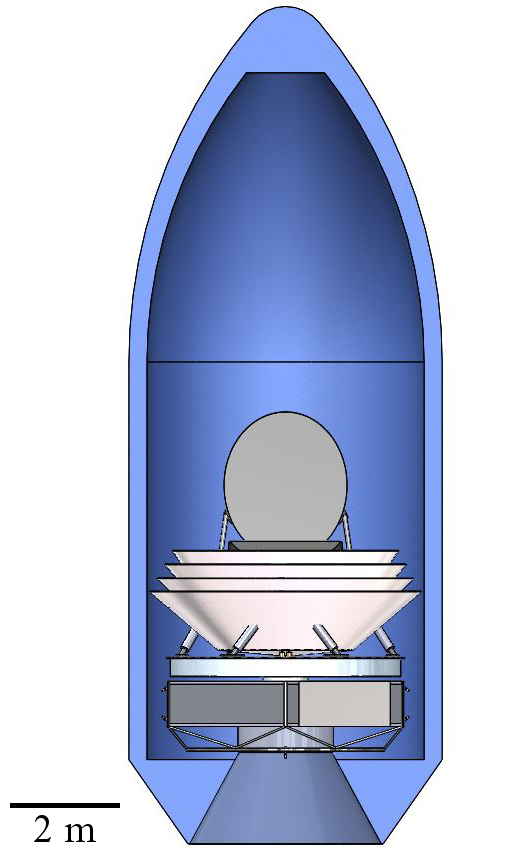
\includegraphics[width=1.5in]{figures/InFairing.JPG}
\caption{\captiontext PICO is compatible with the Falcon~9.\label{fig:InFairing}}
    \end{center}
  \end{minipage}
%
\hfill
\begin{minipage}[b]{0.67\textwidth}
    \begin{center}
    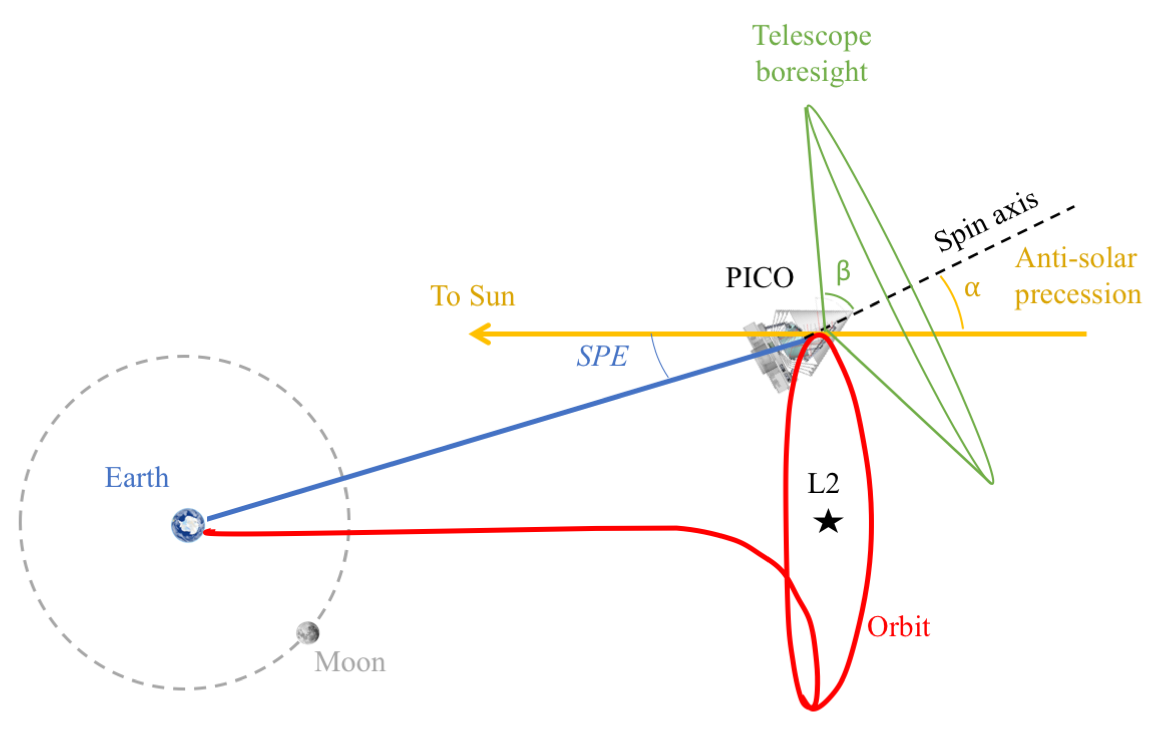
\includegraphics[width=4in]{figures/MissionDesignFigure.png}
\caption{\captiontext
  PICO surveys by continuously spinning the instrument about a
  precessing axis.\label{fig:MissionDesignFigure}}
   \end{center}
  \end{minipage}
 
\end{figure}


% \begin{figure}
% \begin{center}
% 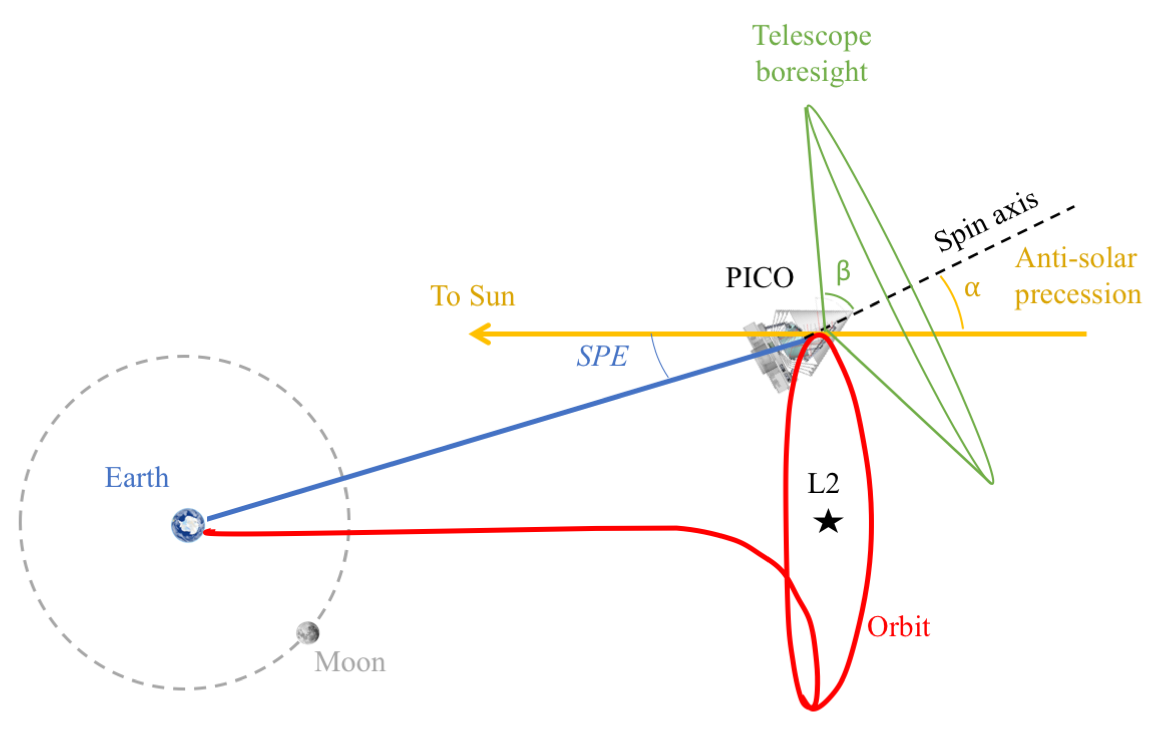
\includegraphics[width=3in]{figures/MissionDesignFigure.png}
% \caption{PICO surveys by continuously spinning the instrument about a
%   precessing axis.\label{fig:MissionDesignFigure}}
% \end{center}
% \end{figure}


% \begin{figure}
% \begin{center}
% 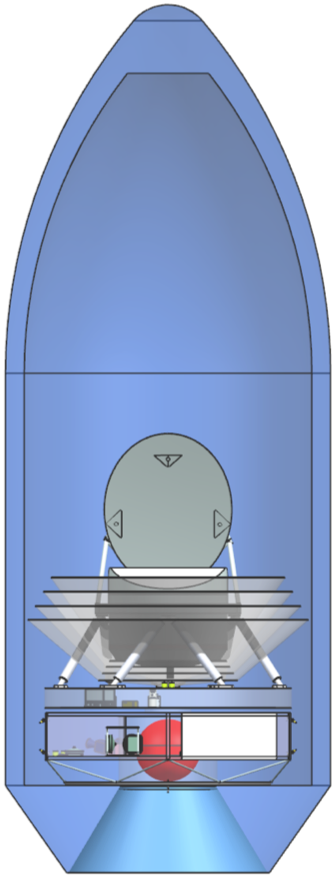
\includegraphics[width=1in]{figures/InFairing.png}
% \caption{PICO is compatible with the Falcon~9.\label{fig:InFairing}}
% \end{center}
% \end{figure}

\subsubsection{Mission Design and Launch}
\label{sec:mission_design} %4.1.1

PICO performs its science survey from a quasi-halo orbit around the
Earth--Sun L2 Lagrange point. Predecessor missions \textit{Planck} and
\textit{WMAP} both operated in L2 orbits.

L2 orbits provide favorable survey geometry (relative to Earth orbits)
by mitigating viewing restrictions imposed by terrestrial and lunar
stray light. The PICO orbit around L2 is small enough to ensure than
the Sun--Probe--Earth (SPE) angle is less than $15\degree$. This
maintains the telescope boresight $>70\degree$ away from the Earth
(Fig.~\ref{fig:MissionDesignFigure},
$70\degree = 180\degree -\alpha - \beta - \rm{SPE}$).

%\input tables/table4.1.tex

High data rate downlink to the Deep Space Network (DSN) is available
from L2 using near-Earth Ka bands. L2 provides a stable thermal
environment, simplifying thermal control. The PICO orbit exhibits no
post-launch eclipses.
 
NASA requires that Probes be compatible with an Evolved Expendable
Launch Vehicle (EELV). For the purpose of this study, the Falcon~9
\citep{SpaceX2015} is used as the reference
vehicle. Figure~\ref{fig:InFairing} shows PICO configured for launch
in a Falcon~9 fairing. The Falcon~9 launch capability for ocean
recovery exceeds PICO's 2147\,kg total launch mass (including contingency) by a
$\sim 50\,\%$ margin.

Insertion to the halo manifold and associated trajectory correction
maneuvers (TCMs) require 150\,m\,s$^{-1}$ of total $\Delta V$ by the
spacecraft. Orbit maintenance requires minimal propellant (statistical
$\Delta V\sim 2$\,m\,s$^{-1}$\,year$^{-1}$). The orbital period is $\sim6$\,months.
There are no disposal requirements for L2 orbits, but spacecraft are customarily
decommissioned to heliocentric orbit.


\subsubsection{Survey Design}
\label{sec:survey_design} %4.1.2
 
PICO employs a highly repetitive scan strategy to map the full
sky. During the survey, PICO spins with a period
$T_{\rm spin} = 1$\,min about a spin axis oriented $\alpha=26\degree$
from the anti-solar direction (Fig.~\ref{fig:MissionDesignFigure}). This spin axis
is forced to precess about the anti-solar direction with a period
$T_{\rm prec}= 10$\,hr. The telescope boresight is oriented at an
angle $\beta=69\degree$ away from the spin axis (Fig.~\ref{fig:InstrumentCAD}). This $\beta$ angle is
chosen such that $\alpha + \beta > 90\degree$, enabling mapping of all
ecliptic latitudes. The precession axis tracks with the Earth in its
yearly orbit around the Sun, so this scan strategy maps the full sky
(all ecliptic longitudes) within 6 months.

PICO's $\alpha=26\degree$ is chosen to be substantially larger than
the \textit{Planck} mission's $\alpha$ angle ($7.5\degree$) to
mitigate systematic effects by scanning across each sky pixel with a
greater diversity of orientations \citep{Hu2003}. Increasing $\alpha$
further would decrease the sun-shadowed volume available for the
optics and consequently reduce the telescope aperture size. A
deployable sun shade was considered but found not to be required, and
was thus excluded in favor of a more conservative and less costly
approach.

The instrument spin rate, selected through a trade study, matches that
of the \textit{Planck} mission. The study balanced low-frequency
($1/f$) noise subtraction (improves with spin rate) against
implementation cost and heritage, pointing reconstruction ability
(anti-correlated with spin rate), and data volume (linearly correlated
with spin rate).  The CMB dipole appears in the PICO data timestream
at the spin frequency (1\,rpm = 16.7\,mHz). Higher multipole signals
appear at harmonics of the spin frequency starting at 33\,mHz, above
the knee in the detector low-frequency noise
(\S\,\ref{sec:sensitivity}). A destriping mapmaker applied in data
post-processing effectively operates as a high-pass filter, as
demonstrated by \textit{Planck} \citep{Kurki-Suonio2009}. PICO's spin
axis precession frequency is $>400\times$ faster than that of
\textit{Planck}, greatly reducing the effects of any residual $1/f$
noise by spreading the effects more isotropically across pixels.

\subsection{Ground Segment}
\label{sec:ground_segment} %4.2

The PICO Mission Operations System (MOS) and Ground Data System (GDS)
can be built with extensive reuse of standard tools. The PICO concept
of operations is described in \S\,\ref{sec:operations}.
% There are
% no time critical events, and no driving data latency
% requirements. Routine orbit maintenance activities are required
% roughly every three months (\S\,\ref{sec:mission_design}). The payload
% consists of a single instrument with a single science observing mode
% (a repetitive survey pattern, \S\,\ref{sec:survey_design}).
All space-ground communications, ranging, and tracking are performed
by the Deep Space Network (DSN) 34\,m Beam Wave Guide (BWG). X-band is
used to transmit spacecraft commanding, return engineering data, and
provide navigation information (S-band is a viable alternative, and
could be considered in a future trade). Ka-band is used for high-rate
return of science data.  The baseline 150\,Mb/s transfer rate
(130\,Mb/s information rate after CCSDS encoding) is an existing DSN
catalog service \cite{DSN2015}.  The instrument produces 6.1\,Tb/day,
which is compressed to 1.5\,Tb/day
(\S\,\ref{sec:detector_readout}). Daily 4\,hr DSN passes return PICO
data in 3.1\,hr, with the remaining 0.9\,hr available as needed for
retransmission or missed-pass recovery.


\begin{figure}
\begin{center}
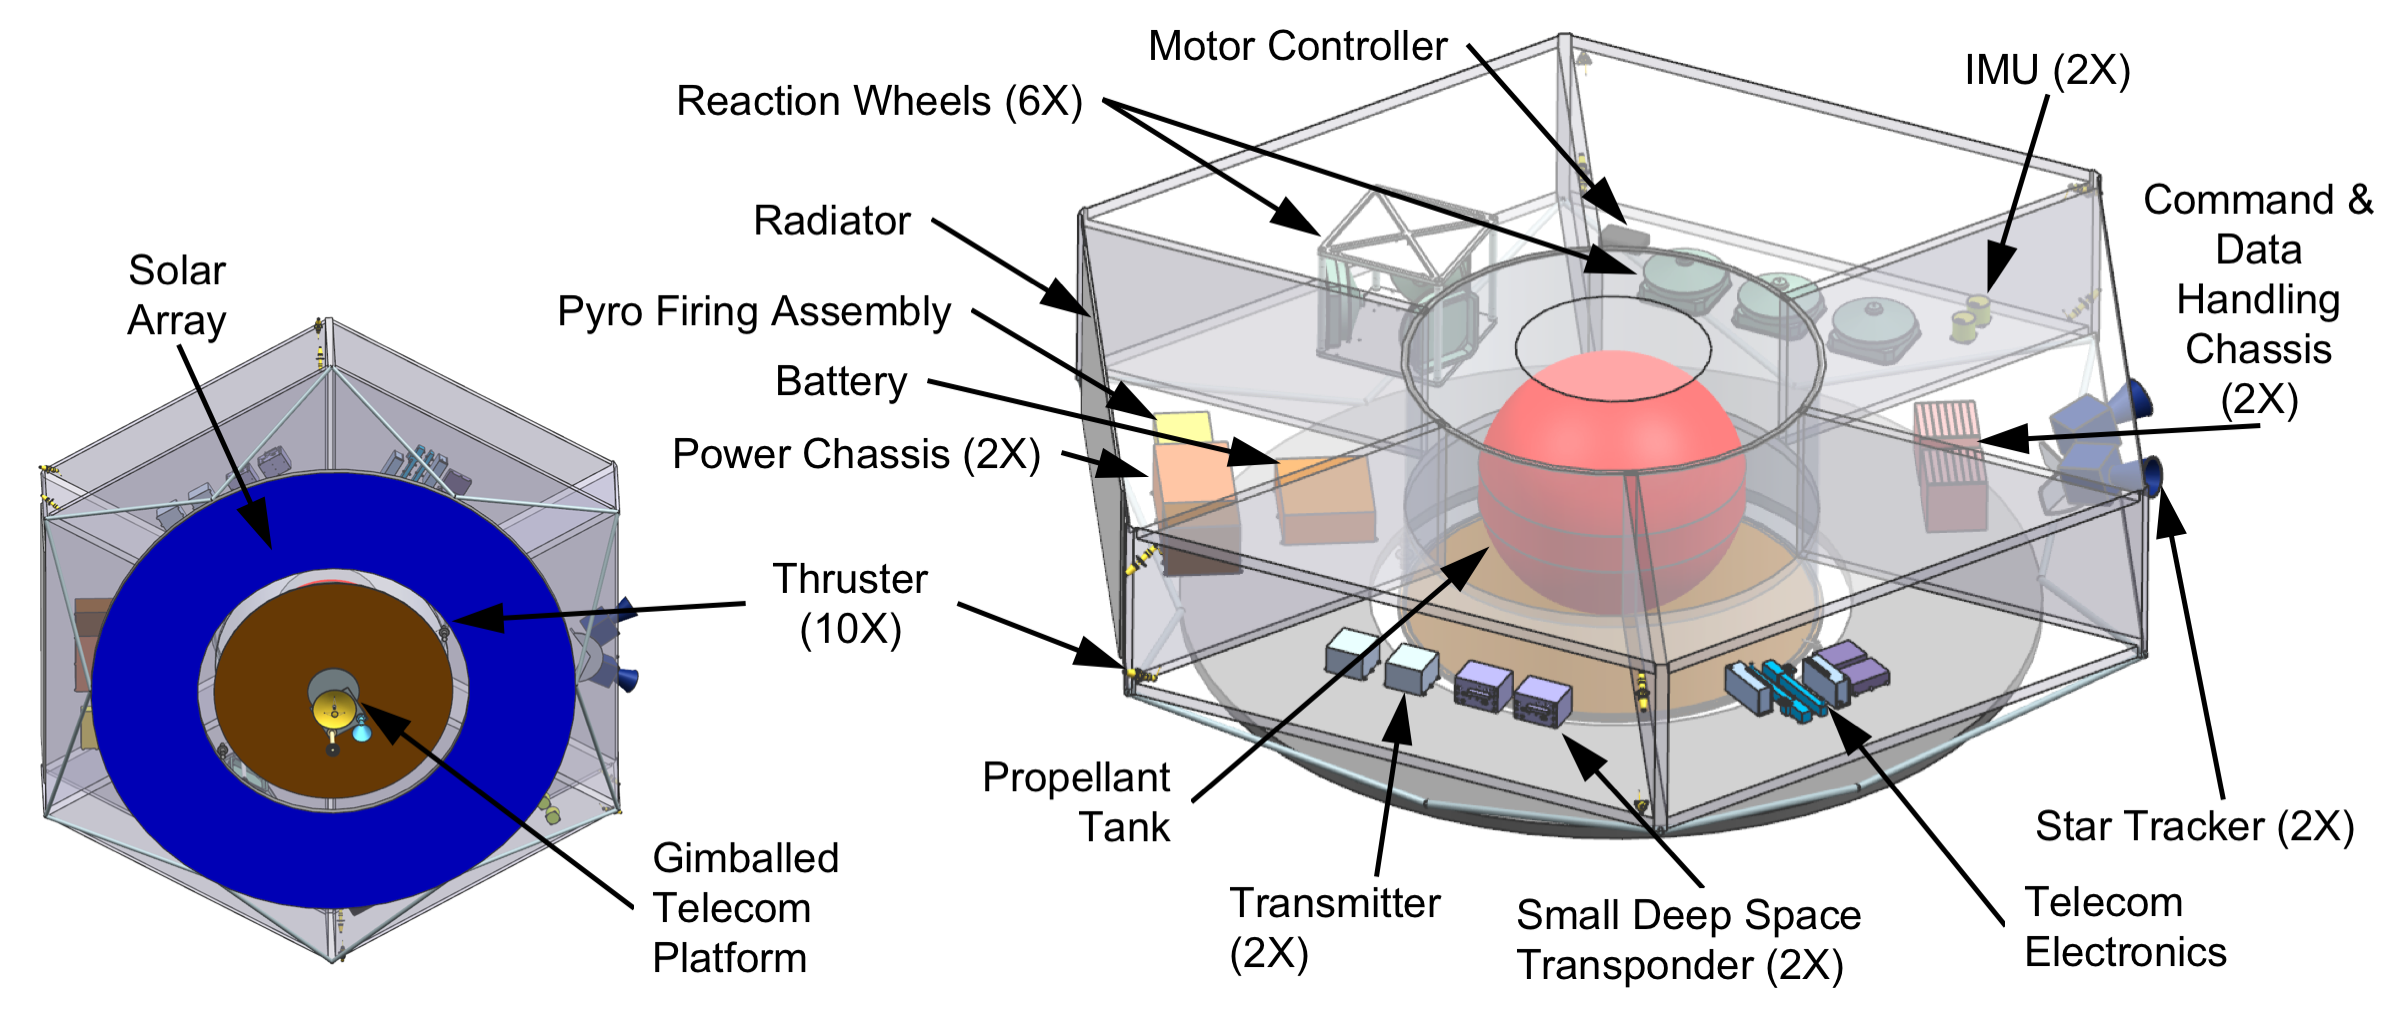
\includegraphics[width=\textwidth]{figures/Spacecraft.png}
\caption{\captiontext
  Modular equipment bays provide easy access to all components
  in the spacecraft de-spun module and enable parallel integration of
  spacecraft subsystems.\label{fig:Spacecraft}}
\end{center}
\end{figure}

\subsection{Spacecraft}
\label{sec:spacecraft} %4.3

The PICO spacecraft bus is Class~B and designed for a minimum lifetime of 5\,years in the L2
environment. Mission critical elements are redundant. Flight spares,
engineering models and prototypes appropriate to Class~B are budgeted.

The aft end of the spacecraft (the ``de-spun module'') is comprised of
six equipment bays that house standard components
(Fig.~\ref{fig:Spacecraft}).  The instrument and V-grooves are mounted on
bipods from the spacecraft ``spun module,'' which contains hosted
instrument elements (Fig.~\ref{fig:InstrumentCAD}). A motor drives the
spun module at 1\,rpm to support the science survey requirements
(\S\,\ref{sec:survey_design}). Reaction wheels on the despun module
cancel the angular momentum of the spun module and provide three-axis
control (\S\,\ref{sec:attitude_determination}).

The bipods that mechanically support the instrument are thermally
insulating. The passively radiating V-groove assembly thermally
isolates the instrument from solar radiation and from the bus
(\S\,\ref{sec:radiative_cooling}). Like \textit{Planck} \citep{Tauber2010}, the V-grooves are
manufactured using honeycomb material. Additional radiators on the
spun and despun spacecraft modules ($\sim1$\,m$^2$ each) reject heat
dissipated by spacecraft subsystems and hosted instrument elements.

PICO's avionics are dual-string with standard interfaces. Solid state
recorders provide three days of science data storage (4.6 Tbit), enabling
retransmission of missed data.

PICO employs a fully redundant Ka- and X-band telecommunications
architecture. The Ka-band system uses a 0.3\,m high-gain antenna to
support a science data downlink information rate of 130 Mb/s to a
34\,m BWG DSN ground station with a link margin of 4.8\,dB. The X-band
system provides command and engineering telemetry communication
through all mission phases using medium and low gain
antennas. Amplifiers, switches, and all three antennas are on a
gimballed platform, enabling Ka and X-band downlink concurrent with
science observations.

 The heritage power electronics are dual-string.
A 74\,A-hr Li-ion battery is sized for a 3\,hr launch phase with 44\,\% depth of discharge.
After the launch phase, the driving
mode is telecom concurrent with science survey (1320\,W including 43\,\% contingency).
Solar cells on the aft side of the bus (5.8\,m$^2$ array, $\alpha=26\degree$ off-Sun) support this mode with positive power,  and unused area in the solar array plane (7.4\,m$^2$ more area by growing to 4.5\,m diameter) affords 125\,\% margin
(Fig.~\ref{fig:Spacecraft}).

The propulsion design is a simple mono-propellant blow-down hydrazine
system with standard redundancy. Two aft-pointed 22\,N thrusters
provide $\Delta V$ and attitude control for orbit insertion and
maintenance (\S\,\ref{sec:mission_design}), requiring 140 kg of
propellant.  Eight 4\,N thrusters provide reaction wheel momentum
management and backup attitude control authority (60\,kg of
propellant). Accounting for ullage (14\,kg), the baseline propellant
tank fill fraction is 77\,\%.


\subsubsection{Attitude Determination and Control}
\label{sec:attitude_determination} %4.3.1

PICO uses a zero net angular momentum control architecture with
heritage from the SMAP mission (\S\,\ref{sec:heritage}). PICO's instrument
spin rate (1\,rpm) matches that of the \textit{Planck} mission, but
the precession of the spin axis is much faster (10\,hr vs 6\, months),
and the precession angle much larger ($26\degree$ vs
$7.5\degree$). These differences make the spin-stabilized
\textit{Planck} control architecture impractical because of the amount
of torque that would be required to drive precession.

The PICO 1\,rpm instrument spin rate is achieved and maintained using
a spin motor. The spin motor drive electronics provide the coarse spin
rate knowledge used for controlling the spin rate to meet the
$\pm0.1$\,rpm requirement. Data and power are passed across the
interface using slip rings.

Based on mass properties derived from the PICO CAD model, PICO
requires $\sim220$\,N\,m\,s to cancel the angular momentum of the
instrument and spacecraft spun module (including mass contingency) at
1\,rpm. Three Honeywell HR-16 reaction wheel assemblies (RWAs), each
capable of 150\,N\,m\,s, are mounted on the despun module parallel to
the instrument spin axis, and spin opposite to the instrument to
achieve zero net angular momentum. The despun module is three-axis
stabilized. The spin axis is precessed using three RWAs mounted normal
to the spin axis in a triangle configuration. Each set of three RWAs
is sized such that two could perform the required function with
margin, providing single fault tolerance.

Spin axis pointing and spin rate knowledge are achieved and maintained
using star tracker and inertial measurement unit (IMU) data. The
attitude determination system is single-fault tolerant, with two IMUs
each on the spun and despun modules, and two star trackers each on the
spun and despun modules. Two sun sensors on the despun module are used
for safe-mode contingencies and instrument Sun avoidance. All attitude
control and reconstruction requirements are met, including spin axis
control $< 60$\,arcmin with $< 1$\,arcmin/min stability, and
reconstructed pointing knowledge $< 10$\,arcsec (each axis, $3\sigma$).

Additional pointing reconstruction is performed in post-processing
using the science data.  The PICO instrument will observe planets
(compact, bright sources) nearly every day.  By fitting the telescope
pointing to the known planetary ephemerides, the knowledge of the
telescope boresight pointing and the relative pointing of each
detector will improve to better than 1\,arcsec (each axis, $3\sigma$). \textit{Planck},
with fewer detectors, making lower signal-to-noise ratio measurements
of the planets, and observing with a scan strategy that acquired
measurements of each planet only once every 6\,months, demonstrated 0.8\,arcsec ($1\sigma$) pointing reconstruction uncertainty in-scan and 1.9\,arcsec ($1\sigma$) cross-scan \citep{2016A&A...594A...1P}.
%(Planck, Planck 2015 results. I. Overview of products and scientific results 2016)

\bigskip
%\newpage
\section{Technology Maturation}
\label{sec:technology_maturation} %5

PICO builds off of the heritage of \planck-HFI and \textit{Herschel}.  Since \planck\ and \textit{Herschel}, suborbital experiments have used monolithically fabricated TES bolometers and multiplexing schemes to field instruments with thousands of \ac{TES} bolometers per camera (Fig.~\ref{fig:spt_fp}). By the time PICO enters Phase~A, the Simons Observatory plans to be operating 60,000 \ac{TES} bolometers~\citep{Simons2018}.

 The remaining technology developments required to enable the PICO baseline design are:
\begin{enumerate}
\item Extension of three-color antenna-coupled bolometers down to 21\,GHz and up to 462\,GHz (\S\,\ref{sec:bolometers}).
\item Construction of high-frequency direct absorbing arrays and laboratory testing (\S\,\ref{sec:dev_arrays}).
\item Beam line and 100\,mK testing to simulate the cosmic ray environment at L2 (\S\,\ref{sec:env_testing}).
\item Expansion of time-division multiplexing to support 128 switched rows per readout column (\S\,\ref{sec:multiplexing}).
%\item Simulation software (\S\,\ref{sec:simulation}). {\color{red}Shaul to fill this in.}
\end{enumerate}
All of these developments are straightforward extensions of technologies already available today.  We recommend APRA and SAT support to complete development of these technologies through the milestones described in Table~\ref{tab:technologies}.


% ------

% PICO's detector and readout technologies have already been
% substantially matured through complementary suborbital experiments,
% and can be developed by the APRA and SAT programs to NASA's Technology
% Readiness Level (TRL)~5 before Phase~A (October 2023) (Table~\ref{tab:technologies}).
% % The 4\,K cryocooler baselined by PICO requires only standard thermal engineering (\S\,\ref{sec:4kcooler}).

% \subsection{Current state of technologies}
% \label{sec:current_state} %5.1

% PICO builds off of the heritage of the \textit{Planck} HFI
% instrument. Since \textit{Planck},
% numerous suborbital experiments have used monolithically fabricated
% TES bolometers and multiplexing schemes to field instruments with
% thousands of detectors per camera (Table~\ref{tab:suborbital})


\subsection{21--462\,GHz Bands}
\label{sec:bolometers} %5.1
%
\begin{wrapfigure}[8]{r}{3.80in}  % r is right aligned, l is left. Capital letters allow figure to float on page.
\vspace{-15pt} % move figure up to align with section headings.
\parbox{2.35in}{
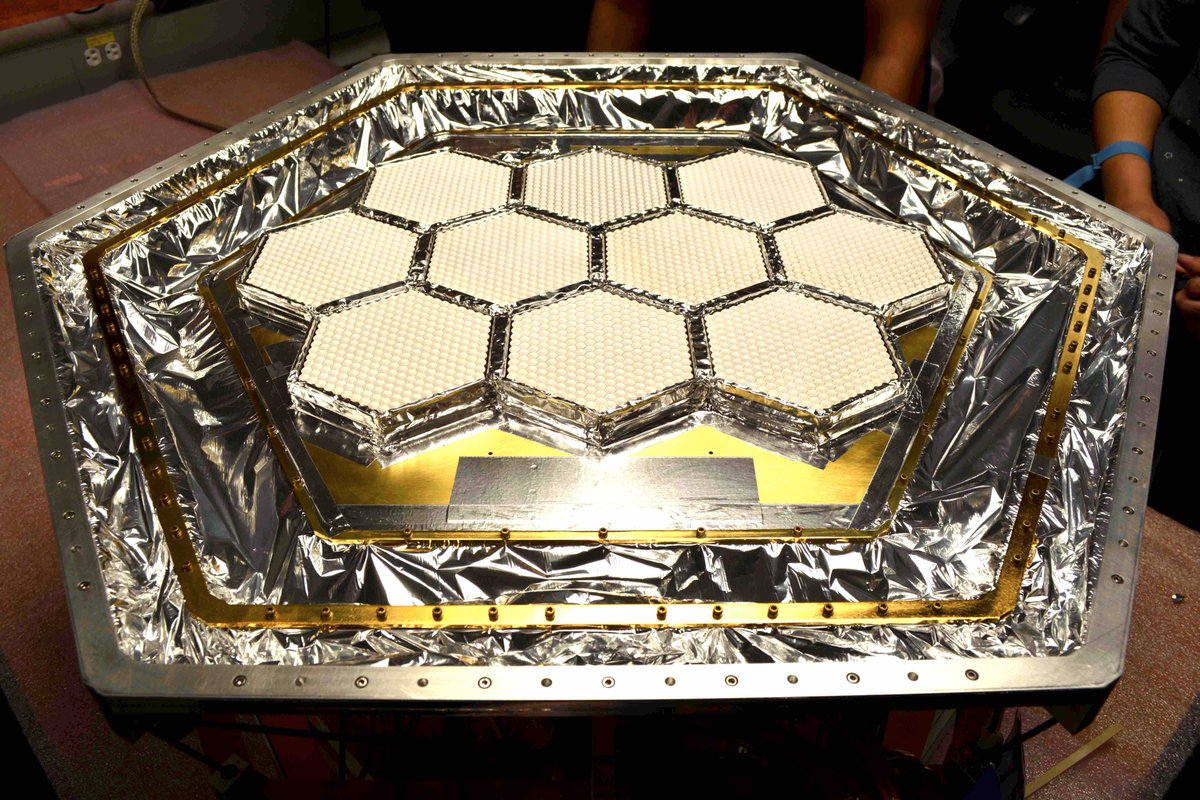
\includegraphics[width=2.35in]{figures/SPT3G.jpg} }  %% image was 3 in wide in past version.
\parbox{1.40in}{
\caption{\captiontext SPT-3G operates a focal plane with sinuous antenna-coupled, three-band pixels with
16,000 bolometers~\citep{Dutcher2018}. Each pixel couples radiation to bands at 95, 150, and
220~GHz.
\label{fig:spt_fp} }
}
\end{wrapfigure}
%
Suborbital teams have successfully demonstrated a variety of optical coupling schemes, including horns with ortho-mode transducers (OMTs), lithographed antenna arrays, and sinuous antennas under lenslets (Table~\ref{tab:suborbital1}). All have achieved background-limited performance in suborbital instruments with sufficient margin on design parameters to achieve this performance in the lower background environment at L2. All have been packaged into modules and focal plane units in working cameras representative of the PICO integration. Experiments have covered many of PICO's observing bands between 27\,GHz and 270\,GHz (Table~\ref{tab:suborbital1}).  To date, suborbital experiments have achieved statistical map depths of 3\,$\mu$K$_{\rm CMB}$\,arcmin on degree-scaled modes over small parts of the sky, within an order of magnitude of what PICO achieves over the entire sky (Table~\ref{tab:bands}), and have demonstrated systematic control better than this level through full-pipeline simulations and null-test analysis (jackknife tests).

% Other experiments have
% successfully deployed two-color pixels. All of these detector arrays
% have been packaged into modules and focal plane units in working
% cameras representative of the PICO integration.

\input tables/table5.1.tex
%\costfootnote

The baseline PICO instrument requires three-color dual-polarized antenna-coupled bolometers covering bands from 21 to 462\,GHz
(\S\,\ref{sec:low_freq_det}).  The sinuous antenna has the bandwidth to service three bands per pixel, whereas horns and antenna arrays have only been used for two. Our baseline is to use a three-band sinuous antenna, although we have a design for PICO that uses two-bands per pixel and has the same baseline noise as PICO~(\S~\ref{sec:technology_descopes}). SPT-3G has used the PICO-baselined three-color pixel design to deploy 16,000 detectors covering 90--150--220\,GHz~\citep{Dutcher2018}.


The extension to lower frequencies requires larger antennas and therefore control of film properties and lithography over larger areas. Scaling to higher frequencies requires tighter fabrication tolerances and materials tend to exhibit higher losses. Current anti-reflection technologies for the lenslets need to be extended with thicker and thinner layers to cover the lowest and highest frequency channels. These developments will require tight control of cleanliness and understanding of process parameters. All developments require careful characterization of beam properties.

\input tables/table5.2.tex

The direction of polarization sensitivity of the sinuous antenna varies with frequency. Over 25\% bandwidth, the variation is approximately $\pm 5$~deg~\citep{obrient2008b}. 
There are potential solutions to this in the focal plane design, measurements, data analysis, and free parameters of the antenna geometry.  A recent study found that pre-flight characterization of the effect through measurements can readily mitigate this systematic effect~\citep{picoweb_wobble}. Systematic effect studies for current field demonstrations, such as with the data of SPT-3G, will be particularly important. The PICO concept is robust to any challenges in developing three-color pixels; 
%  !!!! Paragraph continues after figure!  Difficult tex to force wrapfigure to behave.
%
%
%% figure 5.2 goes with section 5.2, but putting it here to make wrap figure work.  
%
%
\begin{wrapfigure}[27]{r}{0.35\textwidth}  % r is right aligned, l is left. Capital letters allow figure to float on page.
\centering
\vspace{-5pt} % move figure up to align with section headings.
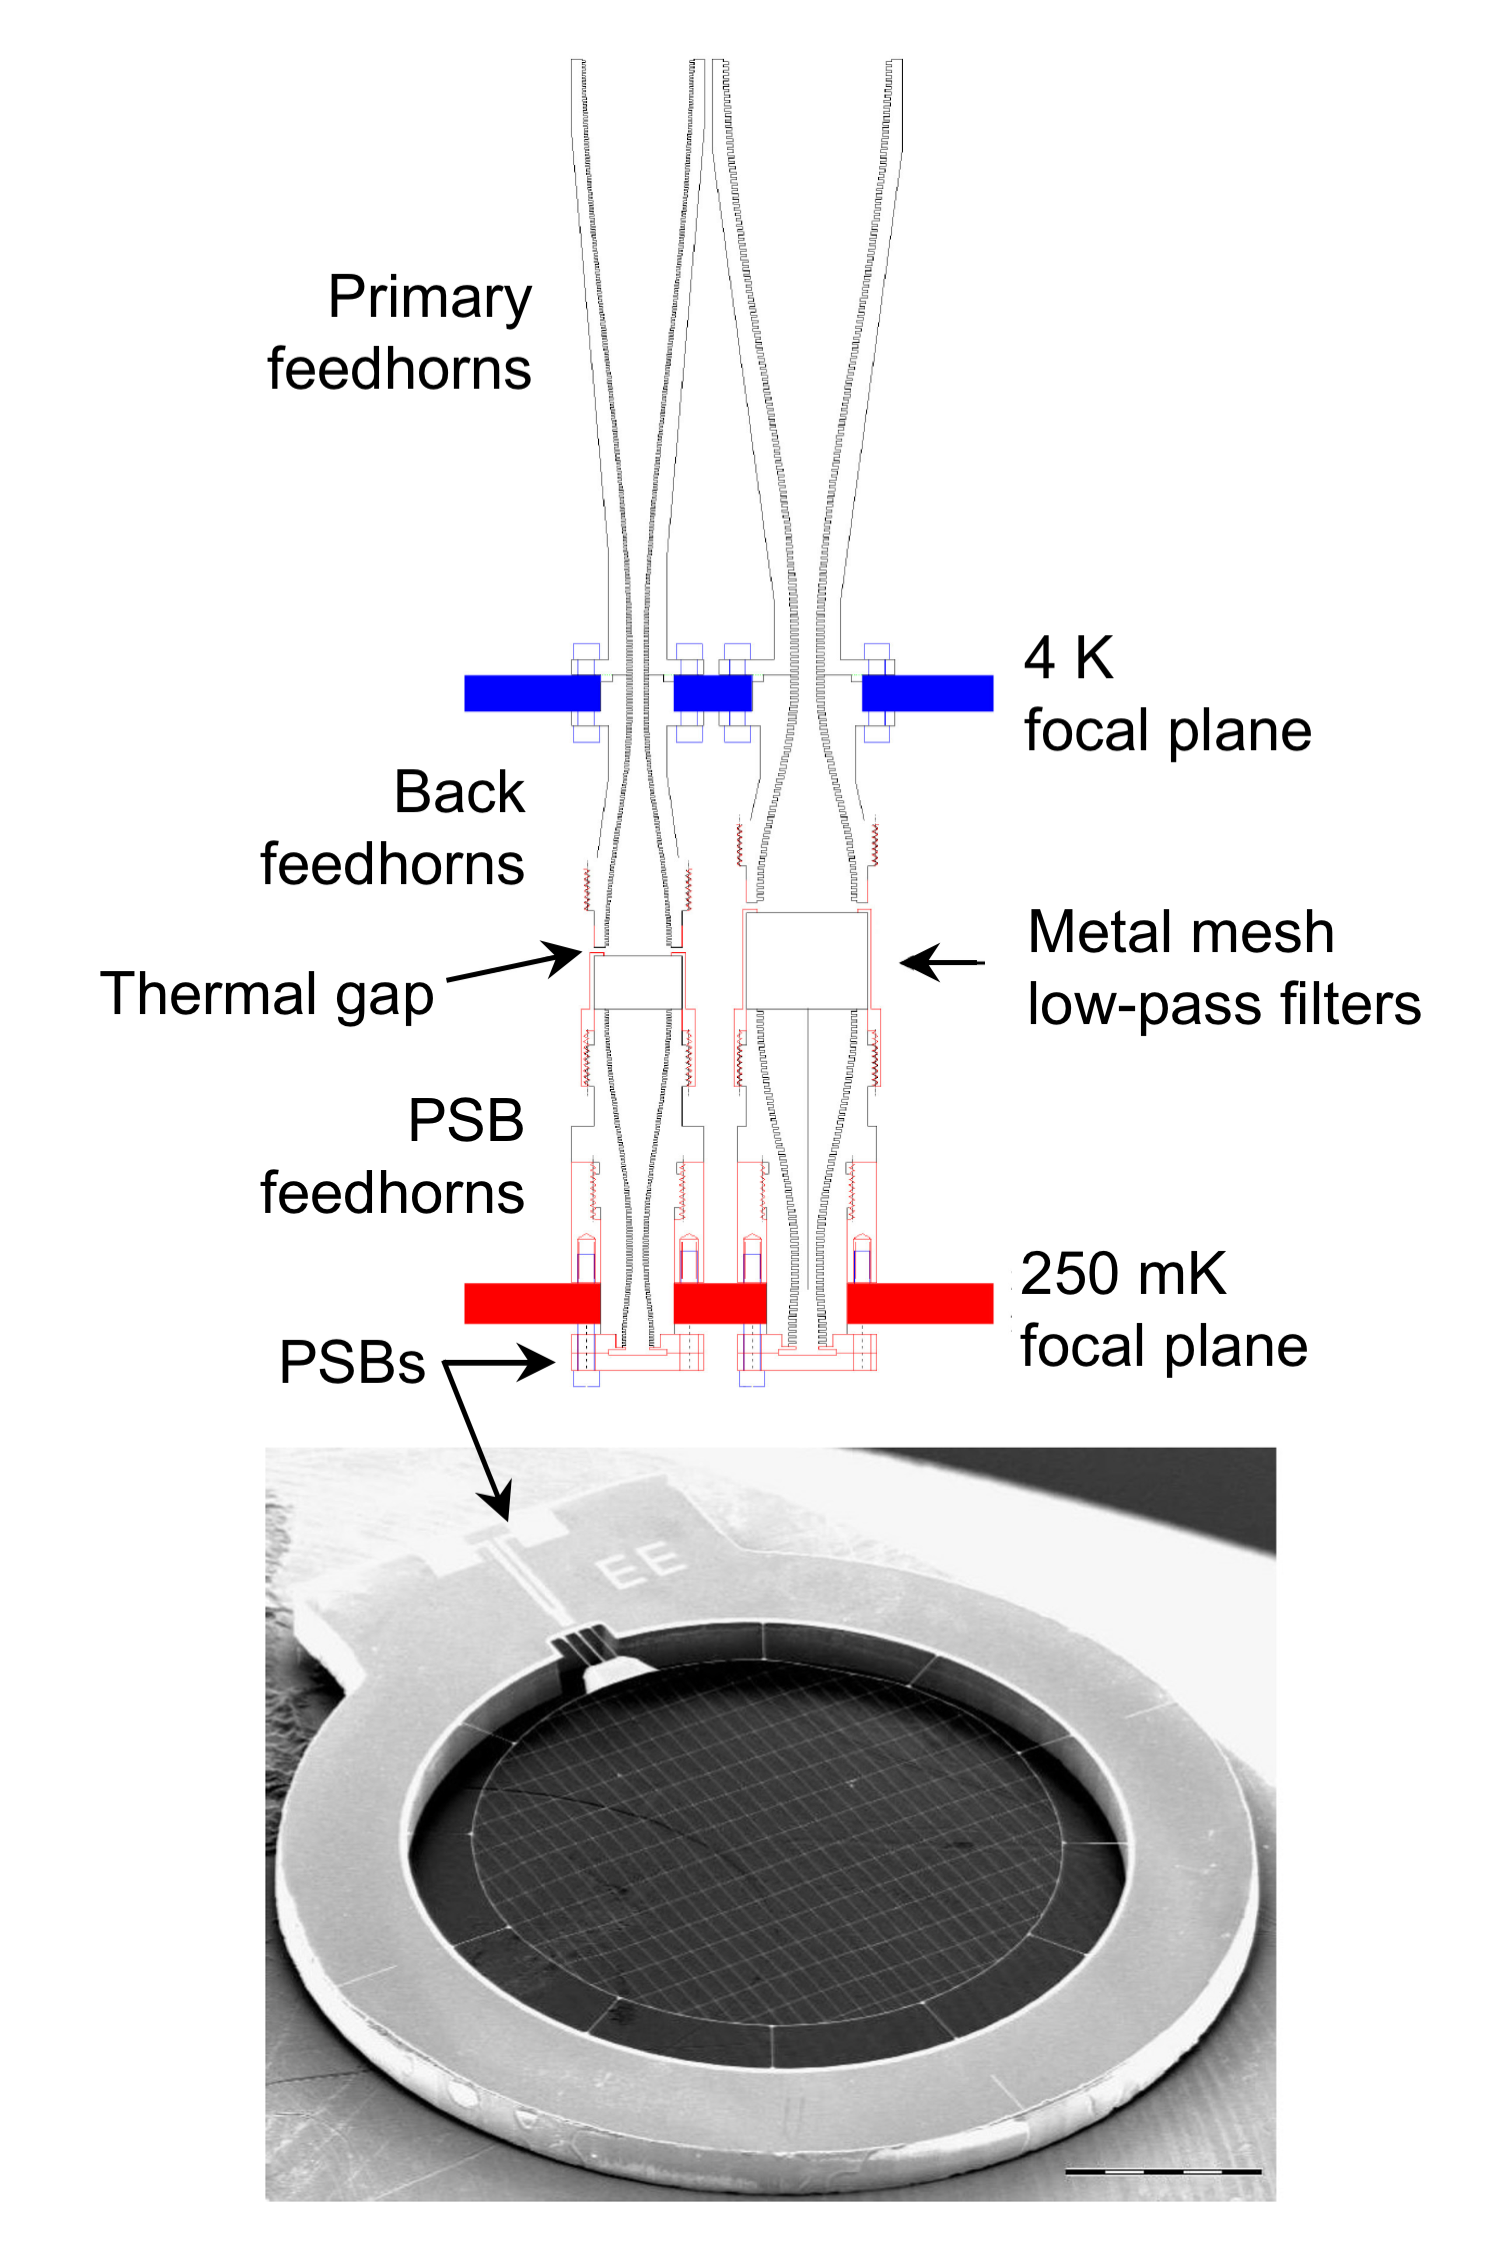
\includegraphics[width=0.35\textwidth]{figures/DirectAbsorbing.png}  %% figure was 2.5 in, .4 /textwidth is 2.6in.
\vspace{-0.25in}
\caption{\captiontext Top: \planck\ used horns to couple the electromagnetic radiation to its detectors. Horn coupling has been used in other experiments, and is the baseline for PICO's coupling between 555 and 799~GHz. Bottom: The photograph shows a dual-polarization, direct-absorbing bolometer from BICEP. The technology was also used with SPT-Pol and \planck-HFI for 143--343\,GHz bands.
\label{fig:DirectAbsorbing} }
\end{wrapfigure}
%
\S\,\ref{sec:technology_descopes} describes an option to descope to two-color horn-coupled pixels, 
a technology with which the polarization sensitivity is constant as a function of frequency.


% \begin{figure}
% \begin{minipage}[b]{0.475\textwidth}
%   \begin{center}
%   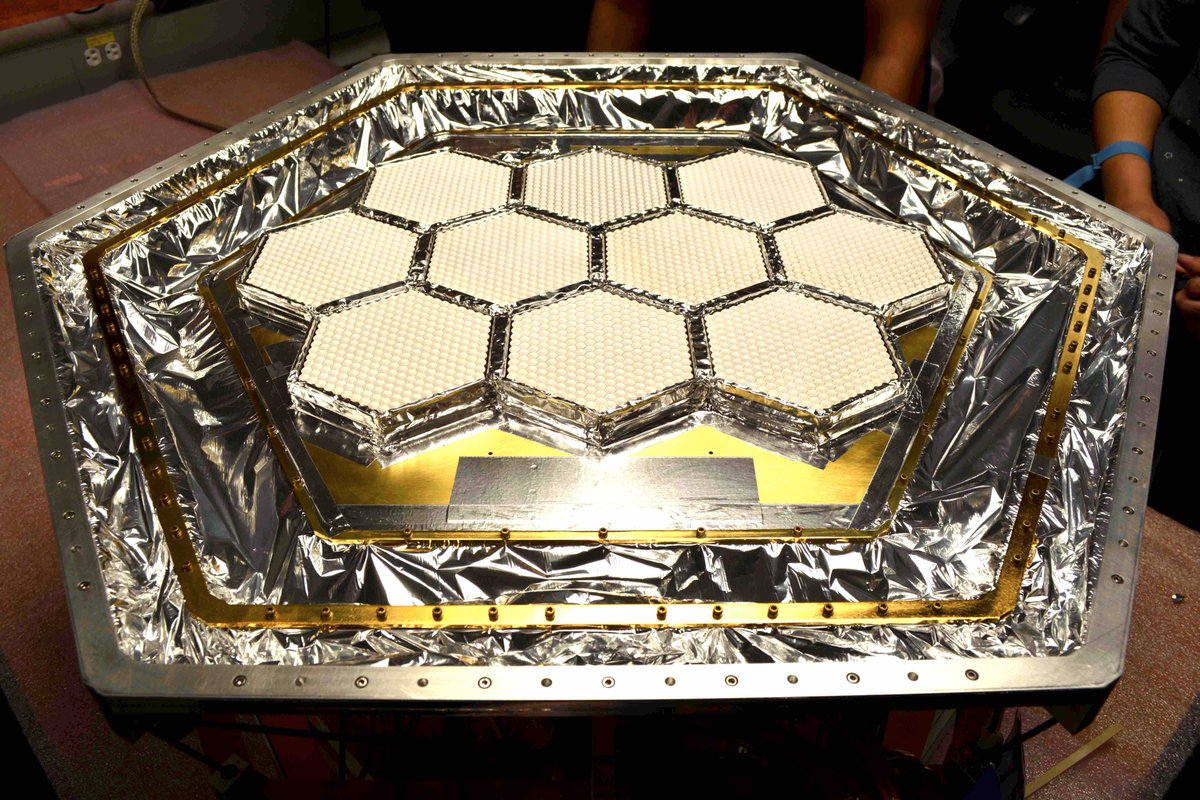
\includegraphics[width=2.5in]{figures/SPT3G.jpg}
%   \caption{\captiontext
%   SPT-3G operates a focal plane with sinuous antenna-coupled, three-band pixels with 16,000 bolometers~\citep{Dutcher2018}. Each pixel couples radiation to bands at 90, 150, and 220~GHz.
%   \label{fig:spt_fp} }
%   \end{center}
%  \end{minipage}
%  \hfill
%   \begin{minipage}[b]{0.475\textwidth}
%     \begin{center}
%     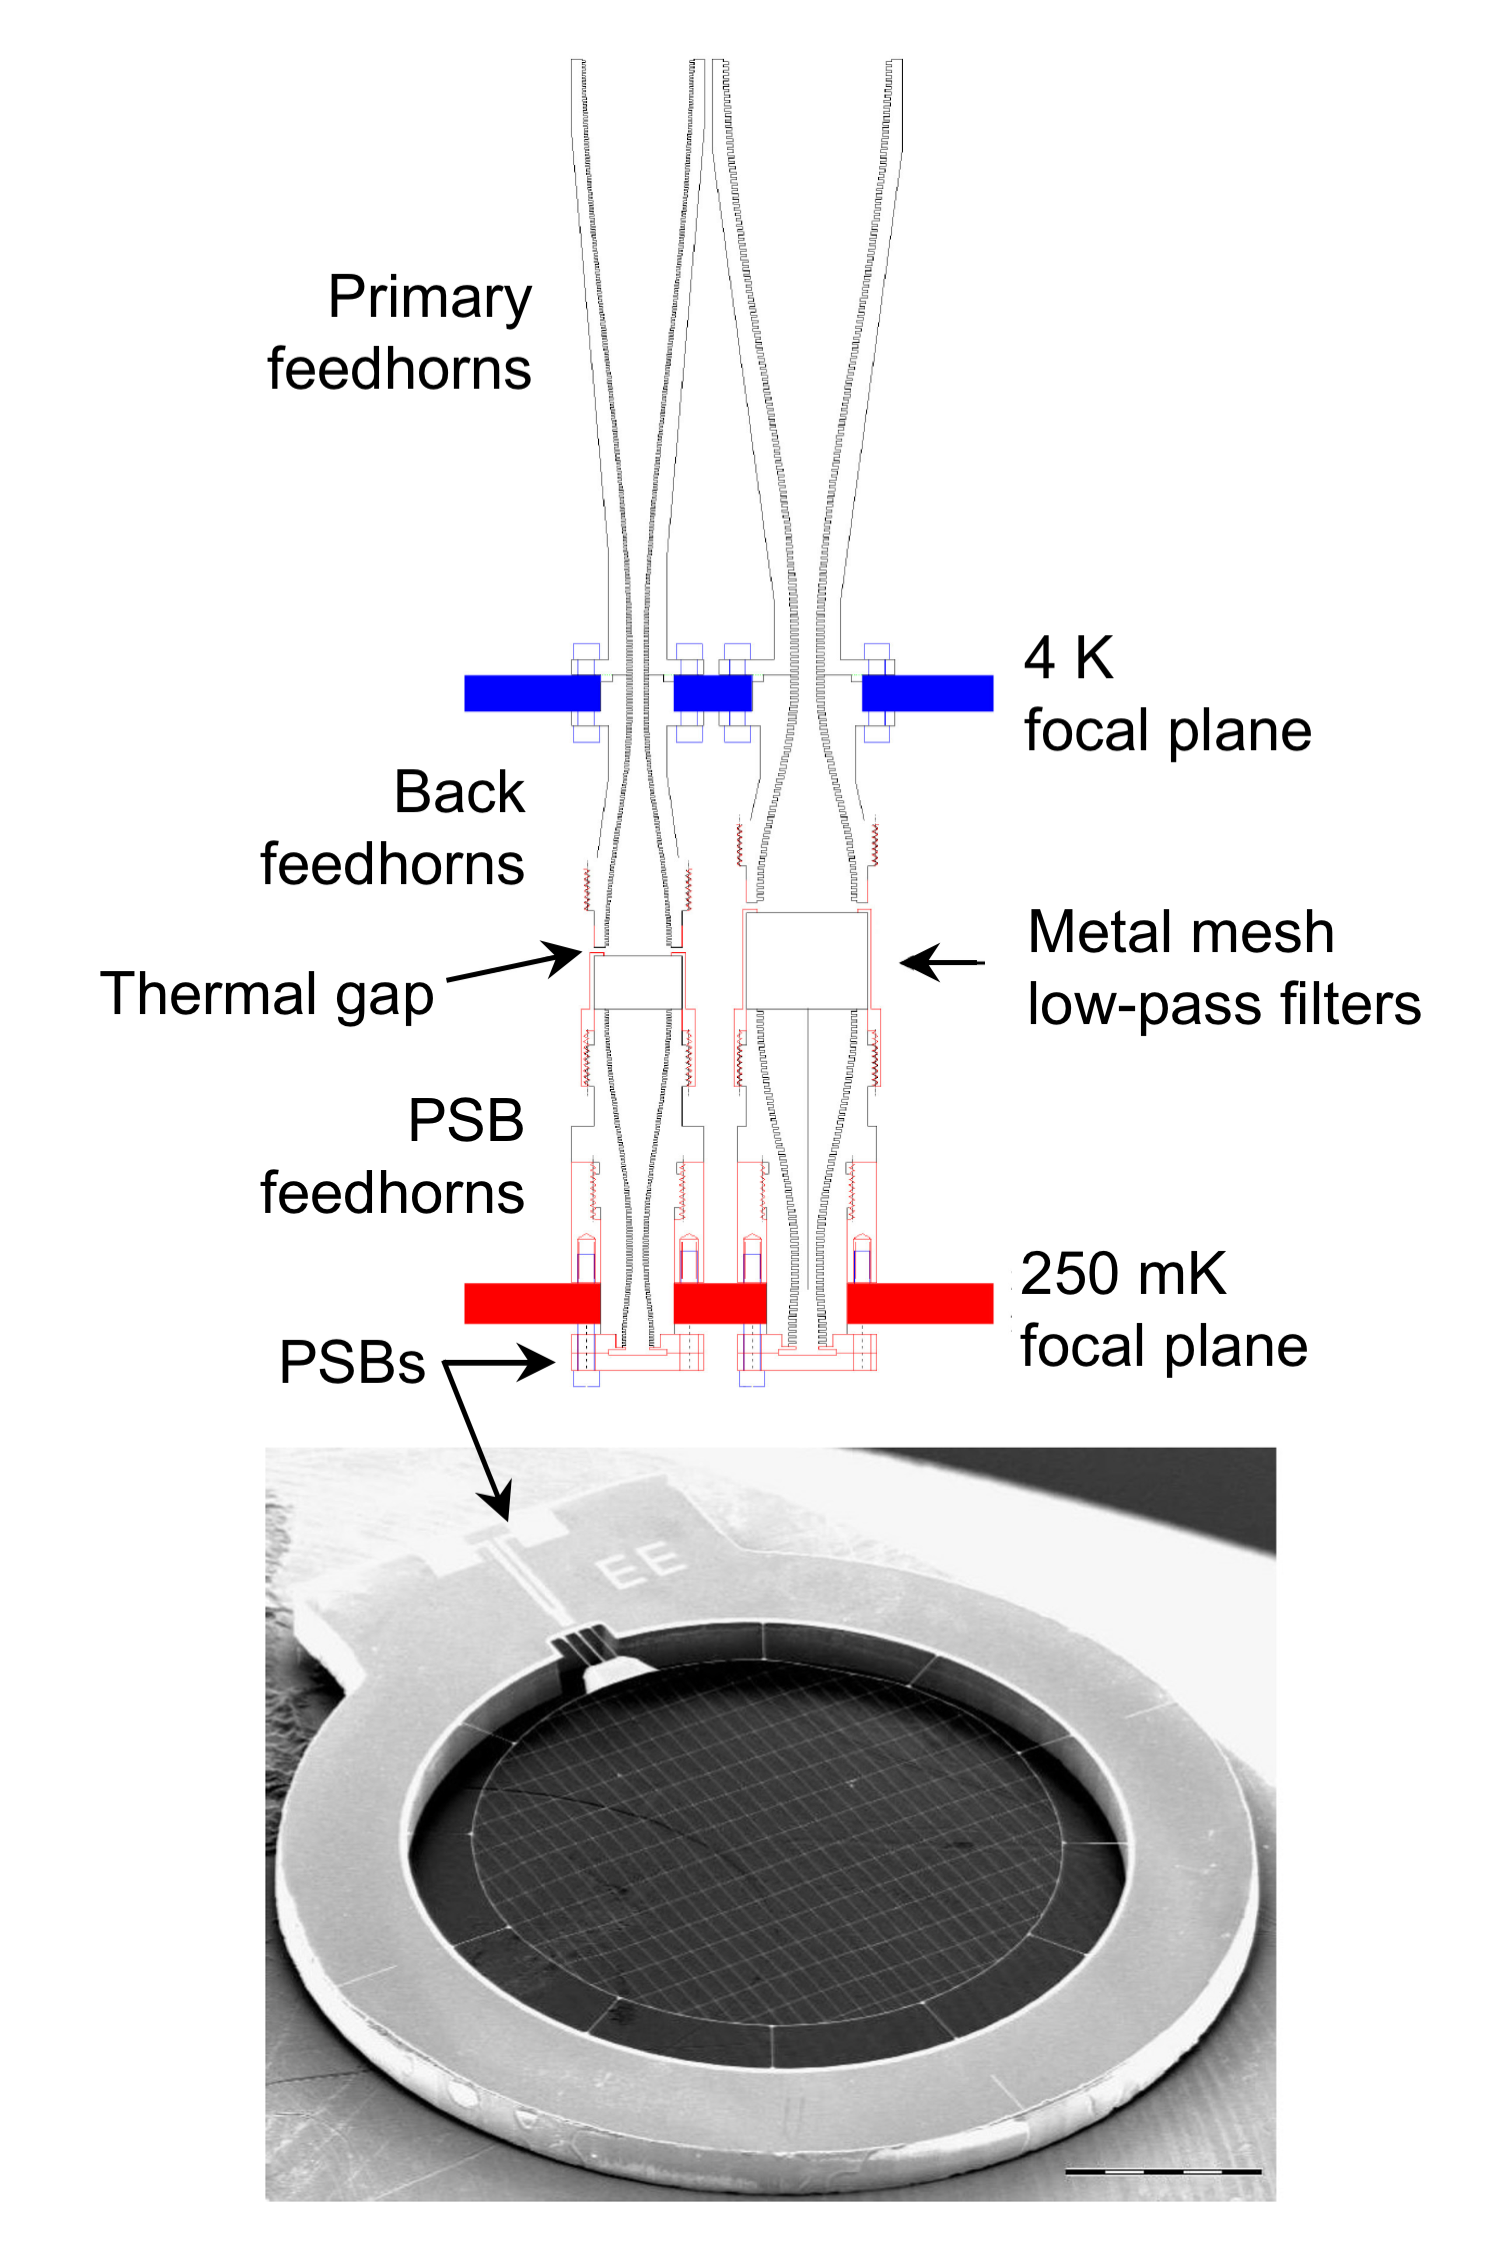
\includegraphics[width=2.5in]{figures/DirectAbsorbing.png}
%     \caption{\captiontext
% Top: \planck\ used horns to couple the electromagnetic radiation to its detectors. Horn coupling has been used in other experiments, and is the baseline for PICO's coupling between 555 and 799~GHz. Bottom: The photograph shows a dual-polarization, direct-absorbing bolometer from BICEP. The technology was also used with SPT-Pol and \planck-HFI for 143--343\,GHz bands.
% \label{fig:DirectAbsorbing} }
%     \end{center}
%   \end{minipage}
% \end{figure}

\subsection{555--799\,GHz bands}
\label{sec:dev_arrays}

The baseline PICO instrument requires single-color, horn-coupled, dual-polarization, direct-absorbing bolometers from 555 to 799\,GHz (\S\,\ref{sec:high_freq_det}).  \planck\ and \textit{Herschel} demonstrated the architecture of horns coupled to direct absorbing bolometers (Fig.~\ref{fig:DirectAbsorbing}).    Ground experiments with similar designs have deployed focal planes with hundreds of horn-coupled spiderweb bolometers, replacing the \textit{Planck} and \textit{Herschel} NTD-Ge thermistors with TESs, and adjusting time constants as necessary (Table~\ref{tab:suborbital2}). \planck -HFI, SPT-pol, and BICEP demonstrated dual-polarized detectors. \textit{Herschel} and SPT-SZ demonstrated monolithic unpolarized detectors. PICO will require detectors that merge these two designs in monolithic dual-polarized arrays. Since all the components of the technology already exist, the remaining necessary development is the packaging. Filled arrays of detectors such as Backshort Under Ground (BUG) bolometers are also an option~\citep{Staguhn2006}.

\input tables/table5.3.tex

%The greatest remaining challenge is the low risk development of a packaging design.

\subsection{Environmental Testing}
\label{sec:env_testing}

Laboratory tests and in-flight data from balloons suggest that TES
bolometer arrays may be more naturally robust against cosmic rays than
the individual NTD-Ge bolometers used in \textit{Planck}. PICO will leverage lessons
learned from \textit{Planck} and ensure robust thermal sinking of
detector array substrates. Cosmic ray
glitches have fast recovery times and low coincidence rates
\citep{SPIDER2018,Filippini_inprep}. Residual risk can be retired with 100\,mK
testing where the array heat sinking may be weaker, and beam-line
tests to simulate the expected flight environment.

\subsection{Multiplexing}
\label{sec:multiplexing}

More than ten experiments have used time-domain multiplexer (TDM)
readout. SCUBA2 on JCMT has 10\,000 pixels, nearly as many detectors
as planned for PICO \citep{Holland2013}. Most of these experiments
have used 32-row multiplexing. Recently ACT has expanded this to
64-row multiplexing \citep{Henderson2016}.

PICO's sensitivity requirements dictate the use of $\sim 13\,000$
transition-edge-sensor bolometers, requiring a highly multiplexed
system.  The PICO baseline design calls for TDM
with 128 switched rows per readout column (TDM-128$\times$). The leap
to TDM-128$\times$ requires:
\begin{itemize}
\item development of fast-switched room temperature electronics; and
\item system engineering of room temperature to cryogenic row select cabling to ensure sufficiently fast row switch settling times.
\end{itemize}

The historical row revisit rate for bolometric instruments using
32$\times$ TDM has been 25\,kHz \cite[e.g.,][]{BICEP2015}. However,
x-ray instruments using TDM routinely switch between rows at a rate of
160\,ns \citep{Doriese2016}. The PICO baseline assumes a 160\,ns
switch rate and TDM-128$\times$, which dictates a row revisit rate
(effective sampling rate) of 48.8\,kHz. To limit aliased noise, PICO
implements L/R filters in each readout channel with a bandwidth of
6\,kHz, dictated by detector stability considerations and the required
$\sim1$\,kHz signal bandwidth.  With these parameters and using the
same TDM multiplexer SQUID design, the increased total noise due to
aliasing will be limited to 15\,\%.  The system engineering study will
culminate in a demonstration of TDM-128$\times$ SQUID aliased noise
below PICO detector sensitivity requirements.


\subsection{Technology Descopes}
\label{sec:technology_descopes} %5.3

A descope from three-color sinuous antenna/lenslet-coupled pixels to two-color horn-coupled pixels remains a viable
alternative should the three-color technology not mature as
planned. Descope studies suggest that a PICO-size focal plane using
two-color horn-coupled pixels at the lower frequencies and the baseline one-color
pixels at the higher frequencies would contain 8,840 detectors
(compared to the baseline 12,966) and map in 19 colors (baseline
21). Because horns have a $2.3:1$ bandwidth, each of the two bands in
a pixel has 35\,\% bandwidth (compared to the baseline 25\,\%), which
compensates for pixel count, resulting in
0.61\,$\mu$K$_{\rm CMB}$\,arcmin aggregate CBE map depth, which
matches the PICO CBE map depth, and affords $>40\,\%$ margin against
the 0.87\,$\mu$K$_{\rm CMB}$\,arcmin baseline requirement
(Table~\ref{tab:bands}), but with coarser spectral resolution.
Detailed analysis could be performed to assess the impact on signal component separation (\S\,\ref{sec:signal_separation}).

\subsection{Enhancing Technologies}
\label{sec:enhancing_technologies} %5.4

The following technologies are neither required nor assumed by the
PICO baseline concept. They represent opportunities to extend
scientific capabilities or simplify engineering.

PICO baselines TDM readout because of its relative maturity and
demonstrated sensitivity and stability in relevant science
missions. Lab tests of Frequency Domain Multiplexing (FDM) suggest
comparable performance with higher multiplexing factors and lower
loads on cryogenic stages relative to TDM. Suborbital experiments such
as SPT-3G have used frequency division multiplexing (FDM) to readout
focal planes comparable in size to PICO.

Microwave frequency SQUID multiplexing can increase the multiplexing
density and reduce the number of lines between the 4\,K and ambient
temperature stages \citep{Dober2017,Irwin2004}. Kinetic Inductance
Detectors (KIDs) and Thermal KIDs (TKIDs) can further reduce the wire
count, obviate the SQUIDs, and dramatically simplify integration by
performing multiplexing on the same substrate as the detectors
themselves \citep{McCarrick2018,Steinbach2018,Johnson2018}. The cost to develop
these technologies is \$3--4M/year, with a high chance of reaching
TRL-5 before Phase~A.
%\costfootnote

%\newpage
%\bigskip
\section{Project Management, Heritage, Risk, and Cost}
\label{sec:project_management} %6

\subsection{PICO Study Participants}
\label{sec:study_participants} %6.1

The PICO study was open to the entire mm/sub-mm science community.
Seven working groups were led by
members of PICO's Executive Committee, which met weekly under the
leadership of PI Shaul Hanany. More than 60 people participated
in-person in two community workshops (November 2017 and May 2018).

The PICO engineering concept definition package was generated by
Team~X (the JPL concurrent design lab). The Team X study was supported
by inputs from a JPL engineering team and Lockheed Martin.

The full list of study report contributors and endorsers is on page~\pageref{authorlist}.

\subsection{Project Management Plan}
\label{sec:management_plan} %6.2

PICO benefits from the experience of predecessor missions such as
\textit{Planck} and \textit{WMAP}, as well as many years of investment
in technology development and a multitude of suborbital
experiments. In addition to demonstrated science and engineering
capabilities, this heritage has developed a community of people with
the expertise required to field a successful mission.

This study assumes mission management by JPL with a Principal
Investigator leading a single science team. A Project Manager provides
project oversight for schedule, budget, and deliverables. A Project
Systems Engineer leads systems engineering activities and serves as
the Engineering Technical Authority. A Mission Assurance Manager
serves as the Independent Technical Authority. The PICO mission
development schedule is shown in Fig.~\ref{fig:Schedule}.

\begin{figure}[hb]
\begin{center}
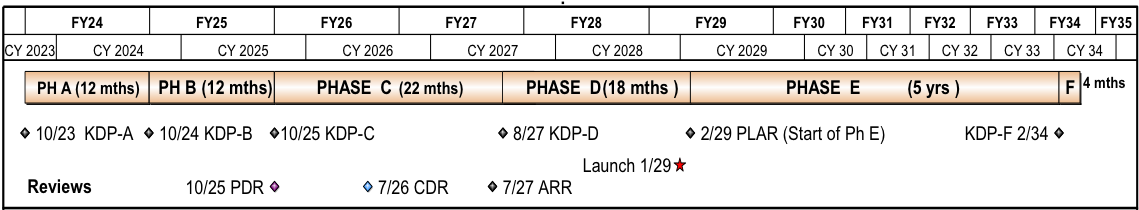
\includegraphics[width=\textwidth]{figures/Schedule.png}
\caption{\captiontext
  The PICO baseline schedule is based on historical actuals
  from similarly-sized missions such as Juno and
  SMAP. Per NASA direction, Probe studies assume a Phase~A start in October 2023.\label{fig:Schedule}}
\end{center}
\end{figure}

Probes are medium-class missions, similar in cost scope to NASA's
New Frontiers missions, which are Category~1 and Risk Classification A
or B, with Phase A--D costs capped at $\sim$ \$850M (not including the
launch vehicle). JPL is well-prepared to manage Probe missions, having
managed the Juno New Frontiers mission (launched 2011) and also the
development of the medium-class \textit{Spitzer} Space Telescope (launched
2003). JPL delivered the bolometric detectors for the \textit{Planck}
HFI instrument (launched 2009). Presently, JPL is managing NEOCam, a
Discovery class infrared space telescope.

The PICO spacecraft provider will be selected during mission
formulation. Multiple organizations are capable of providing a
spacecraft bus to meet PICO's requirements. Lockheed Martin
contributed to the PICO concept study, leveraging their experience
with New Frontiers missions Juno and OSIRIS-REx.
 
\subsection{Heritage}
\label{sec:heritage} %6.3

The successful \textit{Planck} mission provides science heritage for
PICO. Technical heritage traces to multiple missions.

Because PICO observes in the mm/sub-mm regime, the surface accuracy
requirement for the reflectors is relatively easy to meet. PICO's
reflectors are similar to \textit{Planck}'s, but somewhat larger
($270\,{\rm cm} \times 205\,{\rm cm}$ primary vs.\
$189\,{\rm cm} \times 155\,{\rm cm}$)
\citep{Gloesener2006}. \textit{Herschel} observed at wavelengths more
demanding than PICO's and was larger ($350\,{\rm cm}$ diameter
primary) \citep{Toulemont2004}.

The heritage of the PICO detectors and readout electronics
(\S\,\ref{sec:focal_plane}, \S\,\ref{sec:detector_readout}) is
described in \S\,\ref{sec:technology_maturation}.


PICO's detectors are cooled by a cADR (\S\,\ref{sec:cadr}) with
requirements that are within the capabilities of current ADRs
developed by Goddard Space Flight Center. These systems have been
applied to several JAXA missions, including \textit{Hitomi} \citep{Shirron2016}.

PICO's 4\,K cryocooler (\S\,\ref{sec:4kcooler}) is a direct extension
of the JWST MIRI design \citep{Durand2008,Rabb2013}. PICO benefits
from a simpler and more reliable implementation of the J-T system than
was required for MIRI, in that no deployment of cooling lines is
required, and all flow valving is performed on the warm
spacecraft. Cooling multiple independent points with a J-T loop has
been demonstrated on \textit{Planck} with the JPL-supplied 18\,K
cooler \citep{Planck2011}.

Structures similar to PICO's V-groove radiator assembly
(\S\,\ref{sec:radiative_cooling}) are a standard approach for passive
cooling first described more than thirty years ago
\citep{Bard1987}.
%PICO's 4.5\,m diameter V-groove assembly fits inside the launch vehicle fairing.
PICO
has baselined a simple honeycomb material construction like that
successfully flown by the \textit{Planck} mission
\citep{ESA2009,Planck2011}.

Most requirements on the PICO spacecraft are well within typical
ranges and can be met with standard high heritage systems
(\S\,\ref{sec:spacecraft}). PICO's spin architecture and data volume
requirements are less typical, and discussed below.

PICO's spin system is generally less demanding than the successful
SMAP spin system. PICO spins its instrument at 1\,rpm, passes data and
power across the spin interface (Fig.~\ref{fig:ArchitectureBlockDiagram}), and requires $\sim220$\,N\,m\,s of
spin momentum cancellation (\S\,\ref{sec:attitude_determination}). SMAP spins its 6-m instrument
antenna at 14.6\,rpm, successfully passes data and power across the
spin interface, and requires 359\,N\,m\,s of spin momentum cancellation~\citep{Brown2016}.

% The PICO zero-momentum control architecture
% (\S\,\ref{sec:attitude_determination}) has heritage from the SMAP
% mission's successful control architecture. PICO has a slower spin rate and less cancelled angular
% momentum than SMAP. SMAP requires 359\,N\,m\,s to cancel the momentum of a
% 6\,m instrument antenna spun at 14.6\,rpm \citep{Brown2016}.
% Based on mass properties derived from the PICO CAD model, PICO requires XXX N\,m\,s to cancel the momentum of the instrument and spacecraft spun module (XXX\,kg including contingency) at 1\,rpm.
%The PICO launch
% mass (2147\,kg including contingency) is similar to the \textit{Planck} launch mass (1912\,kg \citep{Tauber2010}. If
% we assume \textit{Planck} moments of inertia \citep{ESA2016}, the PICO spun elements
% would have an angular momentum of 210\,N\,m\,s at 1\,rpm. This is
% conservative because, unlike \textit{Planck}, the entire PICO
% observatory does not spin.

Though PICO's data volume is notable by current standards, it is
already enveloped by missions in development. PICO produces
6.1\,Tb/day of raw data which is compressed to 1.5\,Tb/day
(\S\,\ref{sec:detector_readout}). PICO downlinks data daily, but
baselines storage of 3\,days of (compressed) data to mitigate missed
telecom passes. This requires 4.5\,Tb of onboard storage, in family
with the 3.14\,Tb solid state recorder currently in use by Landsat~8
and much smaller than the 12\,Tb flash memory planned for NISAR
\citep{Jasper2017}. The PICO baseline 150\,Mb/s Ka-band data downlink
is an existing DSN catalog service \citep{DSN2015}. The
baseline PICO mission generates $\sim2,200$\,Tb of raw (uncompressed)
data per year, less than the $\sim6,800$\,Tb/year currently returned
by Landsat~8 and $\sim 9,300$\,Tb/yr planned by NISAR
\citep{Jasper2017}.

\subsection{Risk Assessment}
\label{sec:risk_assessment} %6.4

\subsubsection{Pre-Mission Risks}
\label{sec:premission_risks} %6.4.1

Technology development (\S\,\ref{sec:technology_maturation}) is
performed prior to the beginning of mission development, and is
outside of the mission cost (per NASA direction), so associated risks
do not represent threats to the cost of mission development. Rather,
these technology development risks affect
the availability of the described baseline
mission. A technology-related mission descope is described in
\S\,\ref{sec:technology_descopes}.

\subsubsection{Development Risks}
\label{sec:development_risks} %6.4.2

PICO's healthy contingencies, margins, and reserves provide
flexibility to address risks realized during mission development. PICO
carries $>40\,\%$ instrument sensitivity margin (Table~\ref{tab:bands}),
$>100\,\%$ heat lift margin (Table~\ref{tab:cooler}), $43\,\%$ system
power contingency, $31\,\%$ payload mass contingency, and $25\,\%$
spacecraft mass contingency. The Falcon~9 launch capability (assuming ocean
recovery) exceeds PICO's total launch mass (including contingency) by
a $\sim 50\,\%$ margin. The PICO budget includes $30\,\%$ cost
reserves for Phases A--D (\S\,\ref{sec:mission_cost}).

During mission development the Project Systems Engineer continually
assesses risks, tracks progress toward retiring them, and updates
mitigations. Mitigations for a few top risks identified during this
study are described below.
\begin{itemize}
\item Thermal risk can be mitigated through extensive thermal modeling and
review in Phase A, and design for early test verification.
\item Risks
associated with the instrument spin architecture can be mitigated by
engaging JPL engineers who were involved in the SMAP mission.
\item  Detector
delivery schedule risk can be mitigated by beginning fabrication early
in the project life cycle and fabricating a generous number of
detector wafers to ensure adequate yield. Multiple institutions (including, for example, JPL, GSFC, NIST, and ANL) would be capable of producing the PICO detectors. Suborbital programs generally achieve $>66\,\%$ detector wafer yield.
\item Risks associated with the
integration and test of a cryogenic instrument can be mitigated
through advanced planning and allocation of appropriate schedule and
schedule margin.
\end{itemize}

\subsubsection{Operations Risks}
\label{sec:operations_risks} %6.4.3

The PICO design meets the requirements associated with the NASA
Class~B risk classification. For Class~B missions, essential
spacecraft and instrument functions are typically fully
redundant. This increases mission cost, but significantly reduces the
risk of mission failure.

The PICO mission utilizes a single instrument with a single observing
mode mapping the sky using a repetitive survey pattern. The mission
does not require any time-critical activities. The observatory fits in
to the launch vehicle fairing in its operational configuration, so no
hardware deployments are required. Because PICO observes at long
wavelengths, the telescope does not require a dust cover (nor the
associated mission-critical cover release).

The spacecraft incorporates a fault protection system for anomaly
detection and resolution. The Sun-pointed, command receptive,
thermally stable safe-mode attitude allows ground intervention for
fault resolution without time constraints. PICO's high degree of
hardware redundancy and onboard fault protection ensure spacecraft
safety in the event of unforeseen failures and faults.

As described in \S\,\ref{sec:signal_separation} and
\S\,\ref{sec:systematics}, pre-Phase A simulation software maturation
is recommended to mitigate the challenges associated with foreground
separation and systematics control.

%\newpage  % temporay newpage to make wrapfig work and allow better length estimate of document.  to be removed!!

\subsection{Mission Cost}
\label{sec:mission_cost} %6.5
%\costfootnote
%
%\input tables/table6.1-2_vert_wrap.tex
\input tables/table6.1_wrap.tex

We estimate PICO's total Phase A--E lifecycle cost between \$870M and
\$960M, including the \$150M allocation for the Launch Vehicle (per
NASA direction). These cost estimates include 30\,\% reserves for
development (Phases A--D) and 13\,\% reserves for operations
(Phase~E). Pre-Phase-A technology maturation
(\S\,\ref{sec:technology_maturation}) will be accomplished through the
normal APRA and SAT processes, and is not included in the mission cost
(per NASA direction).

Table~\ref{tab:cost} shows the mission cost breakdown, including the
JPL Team~X cost estimate as well as the PICO team cost estimate. Team~X
 is JPL's concurrent design facility. Team~X estimates are generally
model-based, and were generated after a series of instrument and
mission-level studies. Their accuracy is commensurate with the level
of understanding typical to Pre-Phase-A concept development. They do
not constitute an implementation or cost commitment on the part of JPL
or Caltech.

%\input tables/table6.1-2.tex

%\costfootnote

% \begin{table}
% \centering
% \caption{\captiontext
%   Detailed breakdown of Team X and PICO Team cost estimates (in FY18\$). Costs are based on the schedule in Fig.~\ref{fig:Schedule}, which includes 5~years of operations.}\label{tab:cost}
% \footnotesize\rmfamily
% \begin{tabular}{p{2.5in}cc}
% \hline\noalign{\vskip3pt}
% \textbf{Work Breakdown Structure (WBS) Elements}&\textbf{Team~X}&\textbf{PICO Team}\\
% \noalign{\vskip3pt}\hline\noalign{\vskip3pt}
% Development Cost (Phases A--D)&\$724M&\$634M--\$677M\\
% \noalign{\vskip3pt}\hline\noalign{\vskip3pt}
% \quad 1.0, 2.0, 3.0 Management, Systems Engineering, and Mission Assurance&\$54M&\$47M--\$50M\\
% \quad 4.0 Science&\multicolumn{2}{c}{\$19M}\\
% \quad 5.0 Payload System&\multicolumn{2}{c}{\$168M}\\
% \quad 6.0 Flight System&\$248M&\$210M--\$240M\\
% \quad 10.0 Assembly, Test, and Launch Operations (ATLO)&\$24M&\\
% \quad 7.0 Mission Operations Preparation&\multicolumn{2}{c}{\$16M}\\
% \quad 9.0 Ground Data Systems&\multicolumn{2}{c}{\$21M}\\
% \quad 12.0 Mission and Navigation Design&\multicolumn{2}{c}{\$7M}\\
% \quad Development Reserves (30\%)&\$167M&\$146M--\$156M\\
% \noalign{\vskip3pt}\hline\noalign{\vskip3pt}
% Operations Cost (Phase E)&\multicolumn{2}{c}{\$84M}\\
% \noalign{\vskip3pt}\hline\noalign{\vskip3pt}
% \quad 1.0 Management&\multicolumn{2}{c}{\$6M}\\
% \quad 4.0 Science&\multicolumn{2}{c}{\$20M}\\
% \quad 7.0 Mission Operations&\multicolumn{2}{c}{\$34M}\\
% \quad 9.0 Ground Data Systems&\multicolumn{2}{c}{\$14M}\\
% \quad Operations Reserves (13\%)&\multicolumn{2}{c}{\$10M}\\
% \noalign{\vskip3pt}\hline\noalign{\vskip3pt}
% Launch Vehicle Cost&\multicolumn{2}{c}{\$150M}\\
% \noalign{\vskip3pt}\hline\noalign{\vskip3pt}
% Total Cost&\$958M&\$868M--\$911M\\
% \noalign{\vskip3pt}\hline
% \end{tabular}
% \end{table}

The PICO team has generally adopted the Team~X estimates, but also
obtained a parametrically estimated cost range for the Flight System
(WBS 6) and Assembly, Test and Launch Operations (ATLO, WBS~7) from
Lockheed Martin Corporation to represent the cost benefits that might
be realized by working with an industry partner. After adding
estimated JPL overhead and Team~X estimated V-groove assembly costs
(not included in the Lockheed estimate), the PICO team cost is
in-family with but lower than the Team~X cost (Table~\ref{tab:cost}).

Management, Systems Engineering, and Mission Assurance (WBS 1--3)
development costs scale linearly with the WBS 4--12 development costs
in the Team~X model, and are adjusted accordingly in the PICO team
estimate. Science team (WBS~4) costs are assessed by Team~X based on PICO
science team estimates of the numbers and types of contributors and
meetings required for each year of PICO mission development and
operations. These workforce estimates are informed by recent
experience with the \textit{Planck} mission.

Payload system (WBS~5) costs are discussed in detail in
\S\,\ref{sec:instrument_cost}.  PICO's spacecraft (WBS~6) cost
reflects a robust Class~B architecture
(\S\,\ref{sec:spacecraft}). Mission-critical elements are
redundant. Appropriate flight spares, engineering models and
prototypes are budgeted. The V-groove assembly (\S\,\ref{sec:radiative_cooling})
is costed in WBS~6.  Mission operations (WBS~7), Ground Data Systems
(WBS~9), and Mission Navigation and Design (WBS~12) costs reflect a
relatively simple concept of operations (\S\,\ref{sec:operations}). PICO has a single
instrument with a single science observing mode, surveying the sky
continuously using a pre-planned repetitive survey pattern. Orbit
maintenance activities are simple and infrequent.

\subsubsection{Payload Cost}
\label{sec:instrument_cost} %6.5.1

\input tables/table6.2_wrap.tex

The PICO payload consists of a single instrument: an imaging
polarimeter. Payload costs are tabulated in
Table~\ref{tab:instrument_cost}.

%\input tables/table6.2.tex
%\costfootnote
% \begin{table}
% \centering
% \caption{\captiontext  Detailed breakdown of PICO instrument costs.}\label{tab:instrument_cost}
% \footnotesize\rmfamily
% \begin{tabular}{p{2.5in}c}
% \hline\noalign{\vskip3pt}
% \bf  Instrument Elements&\bf Cost\\
% \noalign{\vskip3pt}\hline\noalign{\vskip3pt}
% Management, Systems Eng., Assurance&\$18M\\
% 4\,K Cooler and 0.1\,K cADR&\$71M\\
% Focal plane and electronics&\$27M\\
% Mechanical, Thermal, Software&\$17M\\
% Telescope&\$6M\\
% Instrument integration and test&\$29M\\
% \noalign{\vskip3pt}\hline\noalign{\vskip3pt}
% Total Instrument Cost&\$168M\\
% \noalign{\vskip3pt}\hline
% \end{tabular}
% \end{table}

The superconducting detectors require sub-kelvin cooling to
operate. The active cooling system (the 0.1\,K cADR and 4\,K
cryocooler, \S\,\ref{sec:cadr} and \S\,\ref{sec:4kcooler}) comprises nearly half of the payload
cost. The cADR cost for this study is an estimate from NASA Goddard
Space Flight Center (GSFC), and assumes the provision of both a flight
model and an engineering model. GSFC has produced ADRs for multiple
spaceflight missions. The 4\,K cryocooler cost for this study is based
on the NASA Instrument Cost Model (NICM) VIII CER Cryocooler model
\cite{Mrozinski2017}, assuming a commercial build. PICO benefits
greatly from recent and ongoing investment by commercial suppliers of
4\,K coolers (as described in \S\,\ref{sec:4kcooler}).  Team~X used NICM~VIII to model
the cost of the focal plane and dual string readout electronics (\S\,\ref{sec:focal_plane},
\S\,\ref{sec:detector_readout}).  Team~X estimated the telescope cost using the Stahl model
\cite{Stahl2016}. The telescope is not a major cost driver, primarily
because the reflectors only need to be diffraction limited at 330\,$\mu$m
(900\,GHz) (\S\,\ref{sec:telescope}).

Based on JPL experience, 18\,\% of the instrument cost is allocated
for integration and test. This includes integration and test of the
flight focal-plane assembly with the flight cADR and then integration
and test of the complete instrument including the focal-plane
assembly, reflectors, structures, and coolers (\S\,\ref{sec:iandt}). Integration and
test of the instrument with the spacecraft is costed in WBS~10
(ATLO).
%\costfootnote

\newpage

% [Amy] NASA recently dictated that all Probes add a cost table using
% their standard template. This does not count against the 50 page
% limit. We should paste this in as a graphic rather than converting
% it to a LaTeX table – the whole idea is to standardize, so
% reformatting is not appropriate. The existing cost section (6.5)
% remains (including Table 6.1) – this is an add-on, and should get
% its own page.

\section*{NASA Standard Template Cost Table}

\begin{centering}
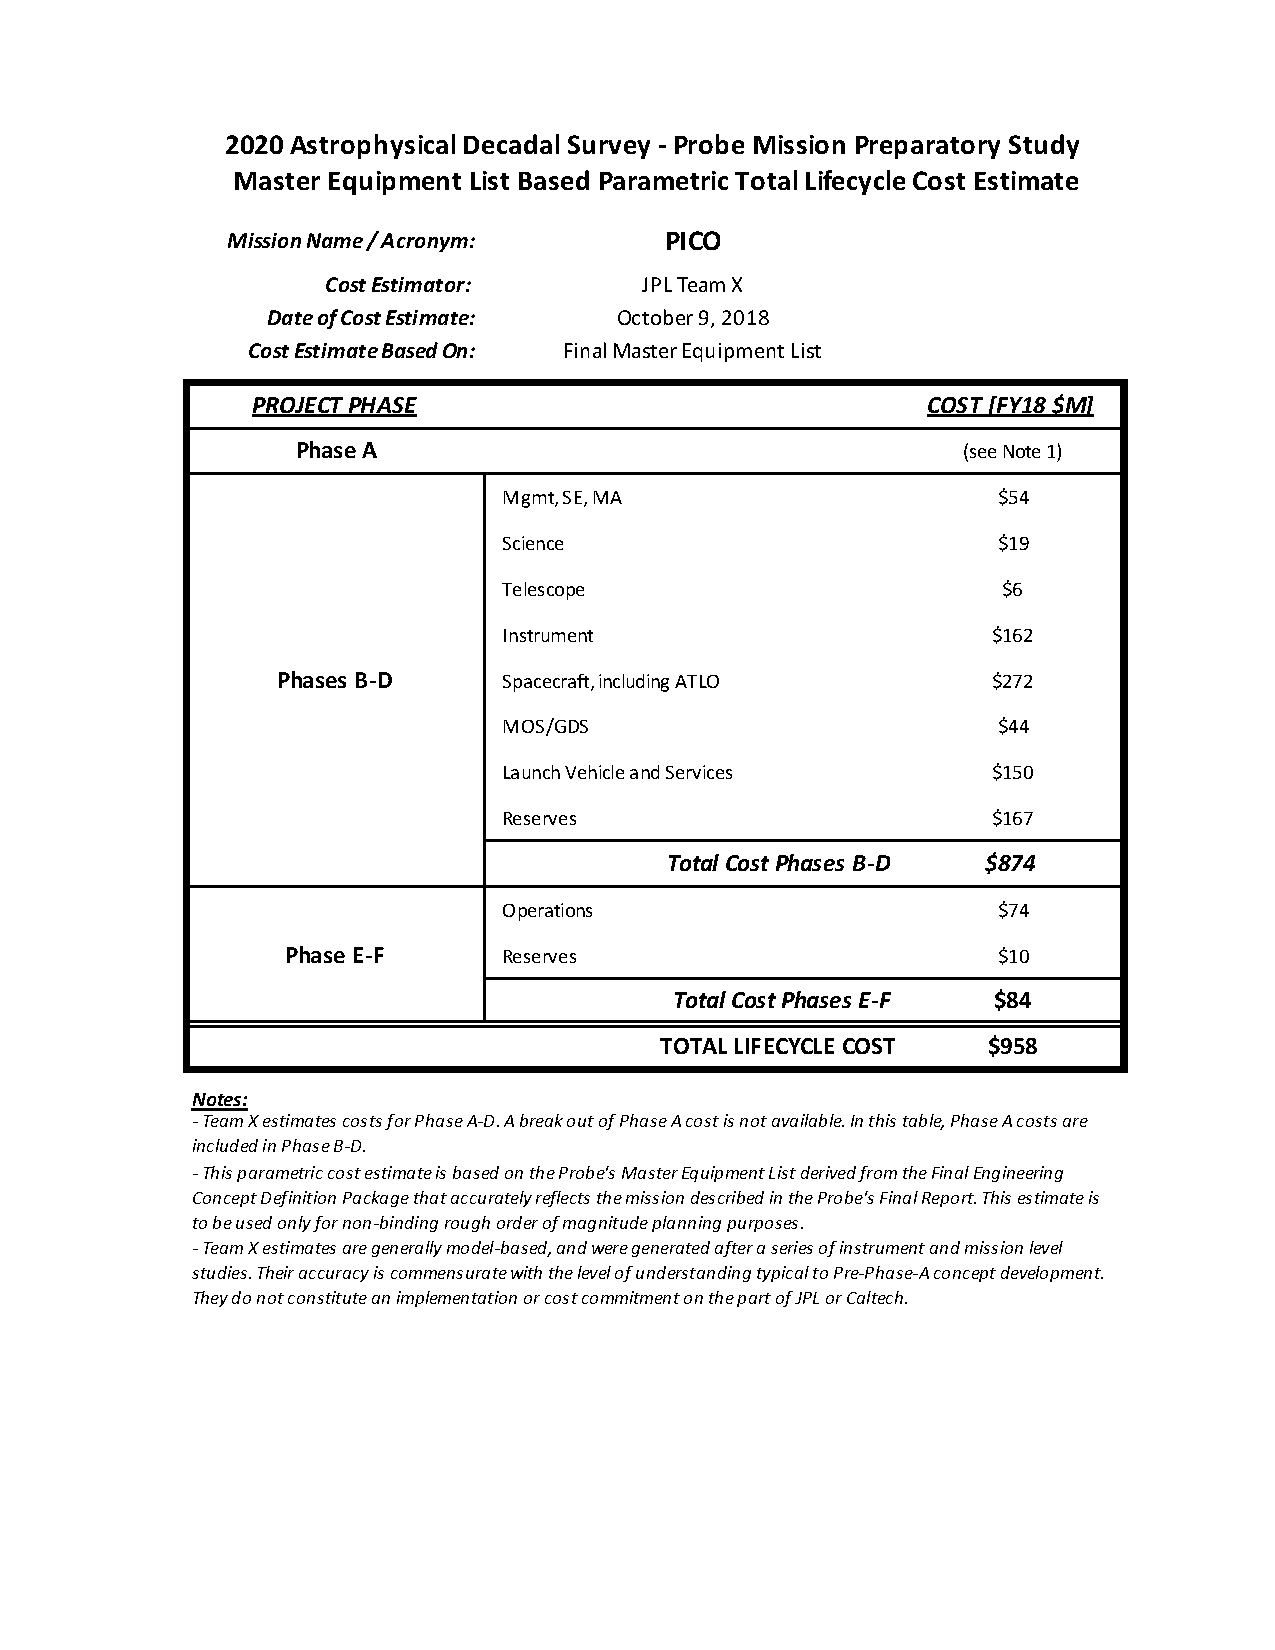
\includegraphics{tables/PICO_Standard_Cost_Table.pdf}
\end{centering}
